%%%%%%%%%%%%%%%%%%%%%%%%%%%%%%%%%%%%%%%%%%%%%%%%%%%%%%%%%%%%%%%%%%%%%%%%%%%%%%%%
% \documentclass[12pt,papel,twoside]{ibtesis}
\documentclass[12pt,screen,twoside,pagebackref]{ibtesis}
% \documentclass[12pt,papel,singlespace,oneside]{ibtesis}
% \documentclass[12pt,papel,preprint,singlespace,oneside]{ibtesis}

%\newcommand{\kari}[1]{\textcolor{red}{#1}}

%%%%%%%%%%%%%%%%%%%%% Paquetes extra %%%%%%%%%%%%%%%%%%%%%%%%%%%%%%%%%%%%%%%%%%%
% Por conveniencia: aqu\'{\i} puede cargar todos los paquetes y definir los comandos 
% que necesite
\usepackage{ibextra}
%%%%%%%%%%%%%%%%%%%%%%%%%%%%%%%%%%%%%%%%%%%%%%%%%%%%%%%%%%%%%%%%%%%%%%%%%%%%%%%%
%%%%%%%%%%%%%%%%%%%%% Informacion sobre la tesis %%%%%%%%%%%%%%%%%%%%%%%%%%%%%%%
\title{Estudio del movimiento de poblaciones animales: redes complejas de interacción inspiradas en datos de campo.}
\author{Marco Madile Hjelt}
\director{Dra. Karina F. Laneri }
\codirector{Dr. Luis G. Moyano}
\carrera{Tesis Carrera de Licenciatura en F\'{\i}sica}
\grado{Licenciando}
\laboratorio{Física Estadística e Interdisciplinaria (FiEstIn) - Centro At\'{o}mico Bariloche}
\jurado{Dr. Marcelo N. Kuperman ~ (Instituto Balseiro)} 
%Dr.~Segundo Jurado (Universidad Nacional de Cuyo)\\ 
%Dr.~J.~Otro Jurado (Univ. Nac. de LaCalle)\\
%Dr.~J.~L\'{o}pez Jurado (Univ. Nac. de Mar del Plata)\\
%Dr.~U.~Amigo (Instituto Balseiro, Centro At\'{o}mico Bariloche)
\palabrasclave{Redes complejas, Chelonoidis chilensis, Uso de refugios}
\keywords{Complex neworks, Chelonoidis chilensis, Burrow use}
% Si queremos poner la fecha manualmente:
% \date{Diciembre de 2099}

%%%%%%%%%%%%%%%%%%%%%%%%%%%%%%%%%%%%%%%%%%%%%%%%%%%%%%%%%%%%%%%%%%%%%%%%%%%%%%%%
%\titlepagefalse % Si no quiere compilar la portada descomente esta linea
%\includeonly{apendices} % Compilar s\'{o}lo estos archivos 
\graphicspath{{figs/}} % Lugar donde encontrar las figuras generales (se puede poner uno en cada cap{\'{\i}}tulo)
%%%%%%%%%%%%%%%%%%%%%%%%%%%%%%%%%%%%%%%%%%%%%%%%%%%%%%%%%%%%%%%%%%%%%%%%%%%%%%%%


\begin{document}

% Dentro del environment 'preliminary' va:
% la dedicatoria, resumen, abstract, indices

\begin{preliminary}

% Escriba su dedicatoria
\dedicatoria{
A Martín y Anna\\
A mis amigos
}

%%% \'{I}ndices %%%%

% \begin{abreviaturas}
%                                 %Abreviaturas
% \end{abreviaturas}

\tableofcontents                %\'{I}ndice

\listoffigures                  %Figuras

\listoftables                   %Tablas

\begin{resumen}%
    A pesar de ser una de las especies más comercializadas en el mercado ilegal de mascotas de Argentina, se conoce muy poco sobre la tortuga 
    terrestre \textit{Chelonoidis chilensis} en su hábitat natural. Debido 
    además a la creciente fragmentación de su hábitat producida principalmente 
    por la reciente introducción de ganado, esta tortuga está catalogada como 
    especie en estado 
    vulnerable. Por estos motivos resulta muy importante el 
    estudio de sus refugios, su área de movimiento y las relaciones entre 
    las tortugas dentro la comunidad. La población de estudio se encuentra 
    en el límite sur de su distribución geográfica, en las cercanías de
    San Antonio Oeste, Patagonia, Argentina. Por ser reptiles se los
    considera 
    solitarios, aunque se sabe muy poco sobre su red de interacción social. 
    En este trabajo, se estudió el movimiento de 27 individuos 
    de \textit{Chelonoidis chilensis} usando dos técnicas de monitoreo: 
    una unidad de navegación  autónoma con GPS y un \textit{datalogger} comercial. 
    Se implementó un método de filtrado de trayectorias y se construyó una 
    grilla de zonas de interés para las tortugas, utilizando las 
    trayectorias filtradas e interpoladas. Se implementaron dos criterios 
    para identificar los refugios nocturnos de las tortugas. Sobre éstos 
    se calculó la distancia media entre refugios y su centro de masa, 
    tanto para machos como para hembras y no se 
    encontraron 
    diferencias significativas en el área abarcada por los refugios para 
    ambos sexos. Se armaron redes bipartitas de nodos 
    tortuga y refugio, y se compararon las proyecciones en nodos tortuga 
    con las redes de interacción diurnas entre pares de tortugas. Se utilizó 
    la proyección en nodos tortuga de 
    la red bipartita como predictor de enlaces en la red de encuentros diurnos
    y se encontró que las predicciones no son estadísticamente significativas. 
    Se calcularon métricas sobre la topología de la red proyectada y no se 
    encontraron diferencias respecto del uso aleatorio de refugios. Finalmente
    , se descubrió la existencia de refugios preferidos y que 
    la tortuga pasa noches consecutivas en refugios geográficamente cercanos.
\end{resumen}

\begin{abstract}%
    Although it is one of the most comercialized species in the Argentinean 
    iligal
    pet market, very little is known about the \textit{Chelonoidis chilensis} 
    tortoise in the wild. This fact, together with the increasing habitat fragmentation 
    produced by cattle, that is being recently introduced into the area, lead to the 
    classification of its conservation status as vulnerable. It is therefore escencial 
    to learn about their burrows, their movement area and the relationship 
    between themselves and within their community. The studied population lives at the
    southernmost distribution of the species, near to San Antonio Oeste city in Patagonia, Argentina. 
    As they are reptiles, they are considered mostly solitary, although very little is 
    known about their social interaction network. In this work, the 
    movement of 27 \textit{Chelonoidis chilensis} tortoises were studied using two monitoring 
    techniques: an autonomous GPS navigation unit and a commercial \textit{datalogger}. A 
    trajectory filtering method was implemented and a grid was built, showing the 
    tortoises's areas of interest. Two criteria were used to identify tortoise nocturnal 
    burrows. The average distance between burrows to the center of mass 
    (of these burrows) was calculated for males and females and no significant differences
    were found. Bipartite networks of tortoise nodes and burrows were built and 
    the projection in tortoise nodes was compared with the diurnal interaction network. The 
    projection 
    in tortoise nodes of the bipartite network was used as a predictor of links 
    in the encounter diurnal network and it was found that the predictions are not 
    statistically significant. Metrics on the topology of the projected network were 
    calculated and no differences were found with respect to the random use of burrows. 
    Finally, the existence of preferred burrows was found and also that tortoises spend
    consecutive nights in nearby burrows.
\end{abstract}


%%% Local Variables: 
%%% mode: latex
%%% TeX-master: "template"
%%% End: 


\end{preliminary}


% Podemos usar cualquiera de los dos comandos: \input o \include para incluir el texto
\chapter{Introducción}
\chapterquote{Avanza rápido el tema de las tortugas}{D. H. Zanette}
 
\section{Motivación}
El movimiento de los animales es de fundamental importancia para procesos ecológicos. Los humanos han estado interesados en el movimiento individual y poblacional por milenios. Hace más de 2000 años, Aristoteles escribió acerca del movimiento de los animales y los conceptos filosóficos y matemáticos asociados, en su libro, \textit{De Motu Animalium.} Históricamente, era crucial entender su comportamiento para saber cómo y dónde se podían obtener estas fuentes de alimento salvajes. Por lo tanto, los primeros humanos eran modeladores naturales del movimiento animal.  En tiempos modernos, estamos interesados en su movimiento por razones científicas y para poder tomar medidas de conservación y protección.
 
 
 
La mayoría de las especies animales son capaces de realizar complejos patrones de movimientos que generalmente dependen del ambiente, factores intrínsecos de los individuos y las interacciones entre ellos (\cite{morales2005adaptive}, \cite{morales2010building} y \cite{nathan2008emerging}). La complejidad de estos movimientos están manifestados en sus trayectorias. %Para el caso de las tortugas estas trayectorias dependen fuertemente de la vegetación en la zona de estudio y la época del año (caso que busquen reproducirse, depositar sus huevos, etc.).
 
 
 
\section{  \textit{Chelonoidis chilensis} }
\label{C chilensis}
 
Nuestra especie de interés es la tortuga $Chelonoidis$ $chilensis$, que se distribuye desde el Gran Chaco hasta el norte de la Patagonia, como se muestra en la Fig.~\ref{fig:distribuciondeEspecie} (\cite{chebez2008se}). Esta especie está incluida en el apéndice de la \textit{Convention on International Trade in Endangered Species of Wild Fauna and Flora (CITES)} y fue categorizada como \textit{vulnerable} a nivel nacional \cite{prado2012categorizacion} e internacional por la \textit{International Union for Conservation of Nature (IUCN)}.
Los principales factores que llevaron a esta situación son la reducción, modificación y destrucción de su hábitat, debido a la expansión de la frontera agropecuaria, así como su comercialización, siendo la especie nativa de reptiles más ilegalmente traficada en el mercado de mascotas en Argentina (\cite{prado2012categorizacion}). Además, la amenaza a esta especie se ve aumentada con la introducción de especies depredadoras exóticas como el Jabalí (\textit{Sus scrofa}) (\cite{kubisch2014chelonoidis}). En este trabajo estudiaremos una población de tortugas en en el límite sur de su distribución geográfica, a 20 km al norte de San Antonio Oeste, provincia de Río Negro, Argentina.  \\
   
Las tortugas son animales  herbívoros que se alimentan con tallos y frutos de cactus (\textit{Opuntia sulphurea, Cereus aethiops, Perocactus tuberosus}), gramíneas (\textit{Chloris castilloniana, Trhichloris crinita}), herbáceas (\textit{Alternanthera pugens, Sphaeralcea miniata, S. mendocina, Portulaca grandiflora}) y vainas de leguminosas (\cite{zacarias2016biologia}).
   
   
   
\begin{figure}[ht]
    \begin{center}
        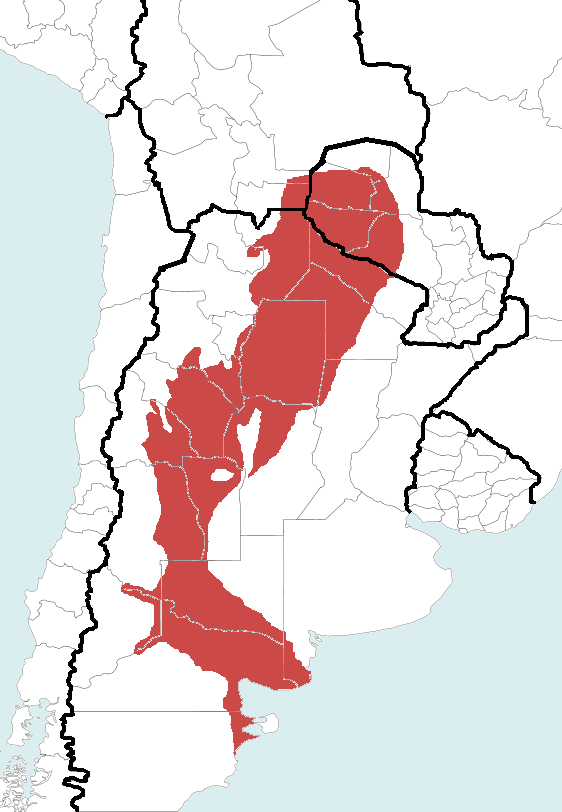
\includegraphics[width=\imsize]{figs/Chap1/Chelonoidis_chilensis_geographic_range.png}
        \caption{Distribución geográfica de la especie de tortuga \textit{Chelonoidis chilensis}
        \label{fig:distribuciondeEspecie}.}
       
        \end{center}
\end{figure}
Esta especie presenta un dimorfismo sexual cuando son adultos, siendo los machos notablemente más chicos que las hembras. El período de actividad (en la distribución más sur) de la especie a las latitudes de la zona de estudio es el más corto, ya que durante el invierno  bruman (parecido a hibernar) por aproximadamente cinco meses. Sus períodos de actividad comienzan durante la primavera, en el mes de septiembre. Desde noviembre a diciembre, ocurren los apareamientos; y entre enero y marzo es cuando las hembras pasan una gran parte del tiempo buscando un lugar adecuado para enterrar sus huevos \cite{Erika}. Al momento se conoce muy poco sobre la dinámica poblacional de C. \textit{chilensis} presente en Argentina.
 
Motivados por la falta de información, el objetivo de este estudio es caracterizar el movimiento y las interacciones de las tortugas en una de las poblaciones en el límite sur de su distribución geográfica. Aprender acerca del movimiento de los individuos es fundamental para entender su rol ecológico en el ecosistema y para diseñar políticas de conservación de la especie y su hábitat.
 
 
\section{Metodologías}
 
Se combinaron diferentes técnicas para monitorear las trayectorias de las tortugas. Para este trabajo se utilizaron datos recolectados por  el grupo de investigación (Física Estadística e Interdisciplinaria) en cuatro campañas de medición realizadas entre enero de 2020 y mayo del 2022.
 
En primer lugar se utilizó la técnica de radiotelemetría para la localización de la posición de las tortugas. En segundo lugar, se utilizó una unidad de navegación (construída en el Centro Atómico Bariloche), para registrar señales de GPS y contaba con sensores inerciales y de temperatura. En tercer lugar, más recientemente en el año 2022 se comenzó a utilizar un datalogger comercial (i-gotU GT120) que toma datos de GPS y hora. En las siguientes subsecciones se proveerán más detalles de ambas metodologías.
 
\subsection{Radiotelemetría}
La técnica de radiotelemetría permite localizar individuos mediante un sistema de transmisor-receptor-antena. Se utilizaron transmisores Holohil (Grand HOLOHIL Systems Ltd. RI-2B) pegados a los caparazones de las tortugas mediante cinta adhesiva. Estos transmisores emiten un pulso a una determinada frecuencia ($\approx$150 MHz) cada dos segundos. Los pulsos eran detectados por un sistema de recepción, que consiste en una antena Yagi-Uda conectada a un receptor ATS R410 (Advanced Telemetry Systems,Inc). Esta técnica permite con gran precisión localizar el transmisor y, usando un GPS portátil (Garmin eTrex
x20), determinar la ubicación de la tortuga.
 
A pesar de ser muy precisa espacialmente, esta técnica no posee una buena resolución temporal, necesaria para reconstruir trayectorias confiables. En primer lugar, es necesario seguir constantemente al individuo para tener una mejor resolución temporal. En segundo lugar, el investigador debe acercarse a una distancia considerable de la tortuga para tomar su posición con el GPS. Ambos factores pueden alterar el comportamiento de la tortuga y su trayectoria. En la siguiente sección se describe la unidad de navegación, que ofrece una alta resolución temporal en las trayectorias sin perturbar al comportamiento animal. Es por esta razón que solo se usó esta técnica para recuperar la unidad de navegación y el i-gotU, no para monitorear la trayectoría directamente.
 
\subsection{Unidad de navegación}
Se desarrolló en el departamento de Ingeniería del Centro Atómico  una unidad de bajo presupuesto para monitorear individuos en su hábitat natural (de ahora en más llamado tortugómetro), que consiste de un receptor GPS, sensores inerciales (acelerómetro y giróscopo) y un sensor de temperatura (Fig.~\ref{fig:tortugometro}). El mismo está alimentado por una batería recargable que le da una autonomía de aproximadamente 15 horas considerando una adquisición del GPS de un punto cada 5-10 minutos. El peso del tortugómetro es de 45 g representando el 3\% del peso de una tortuga de tamaño medio, lo que es aceptable para no disturbar el movimiento del animal. Los datos del receptor de GPS y de los sensores inerciales son guardados en una memoria micro-SD. Al final de cada día de monitoreo se descargaron los datos de la memoria y se cargaron las baterías.
 
En este trabajo, se utilizaron datos obtenidos por campañas realizadas por el grupo de investigación. Se contó con 8 de estas unidades en correcto funcionamiento para monitorear las tortugas en cada día de campaña. Las campañas de medición donde se utilizó esta técnica fueron entre enero de 2020 y enero del 2022. Se monitorearon en total 27 individuos por un total de 1160 horas.
\begin{figure}[ht]
    \begin{center}
       
   
    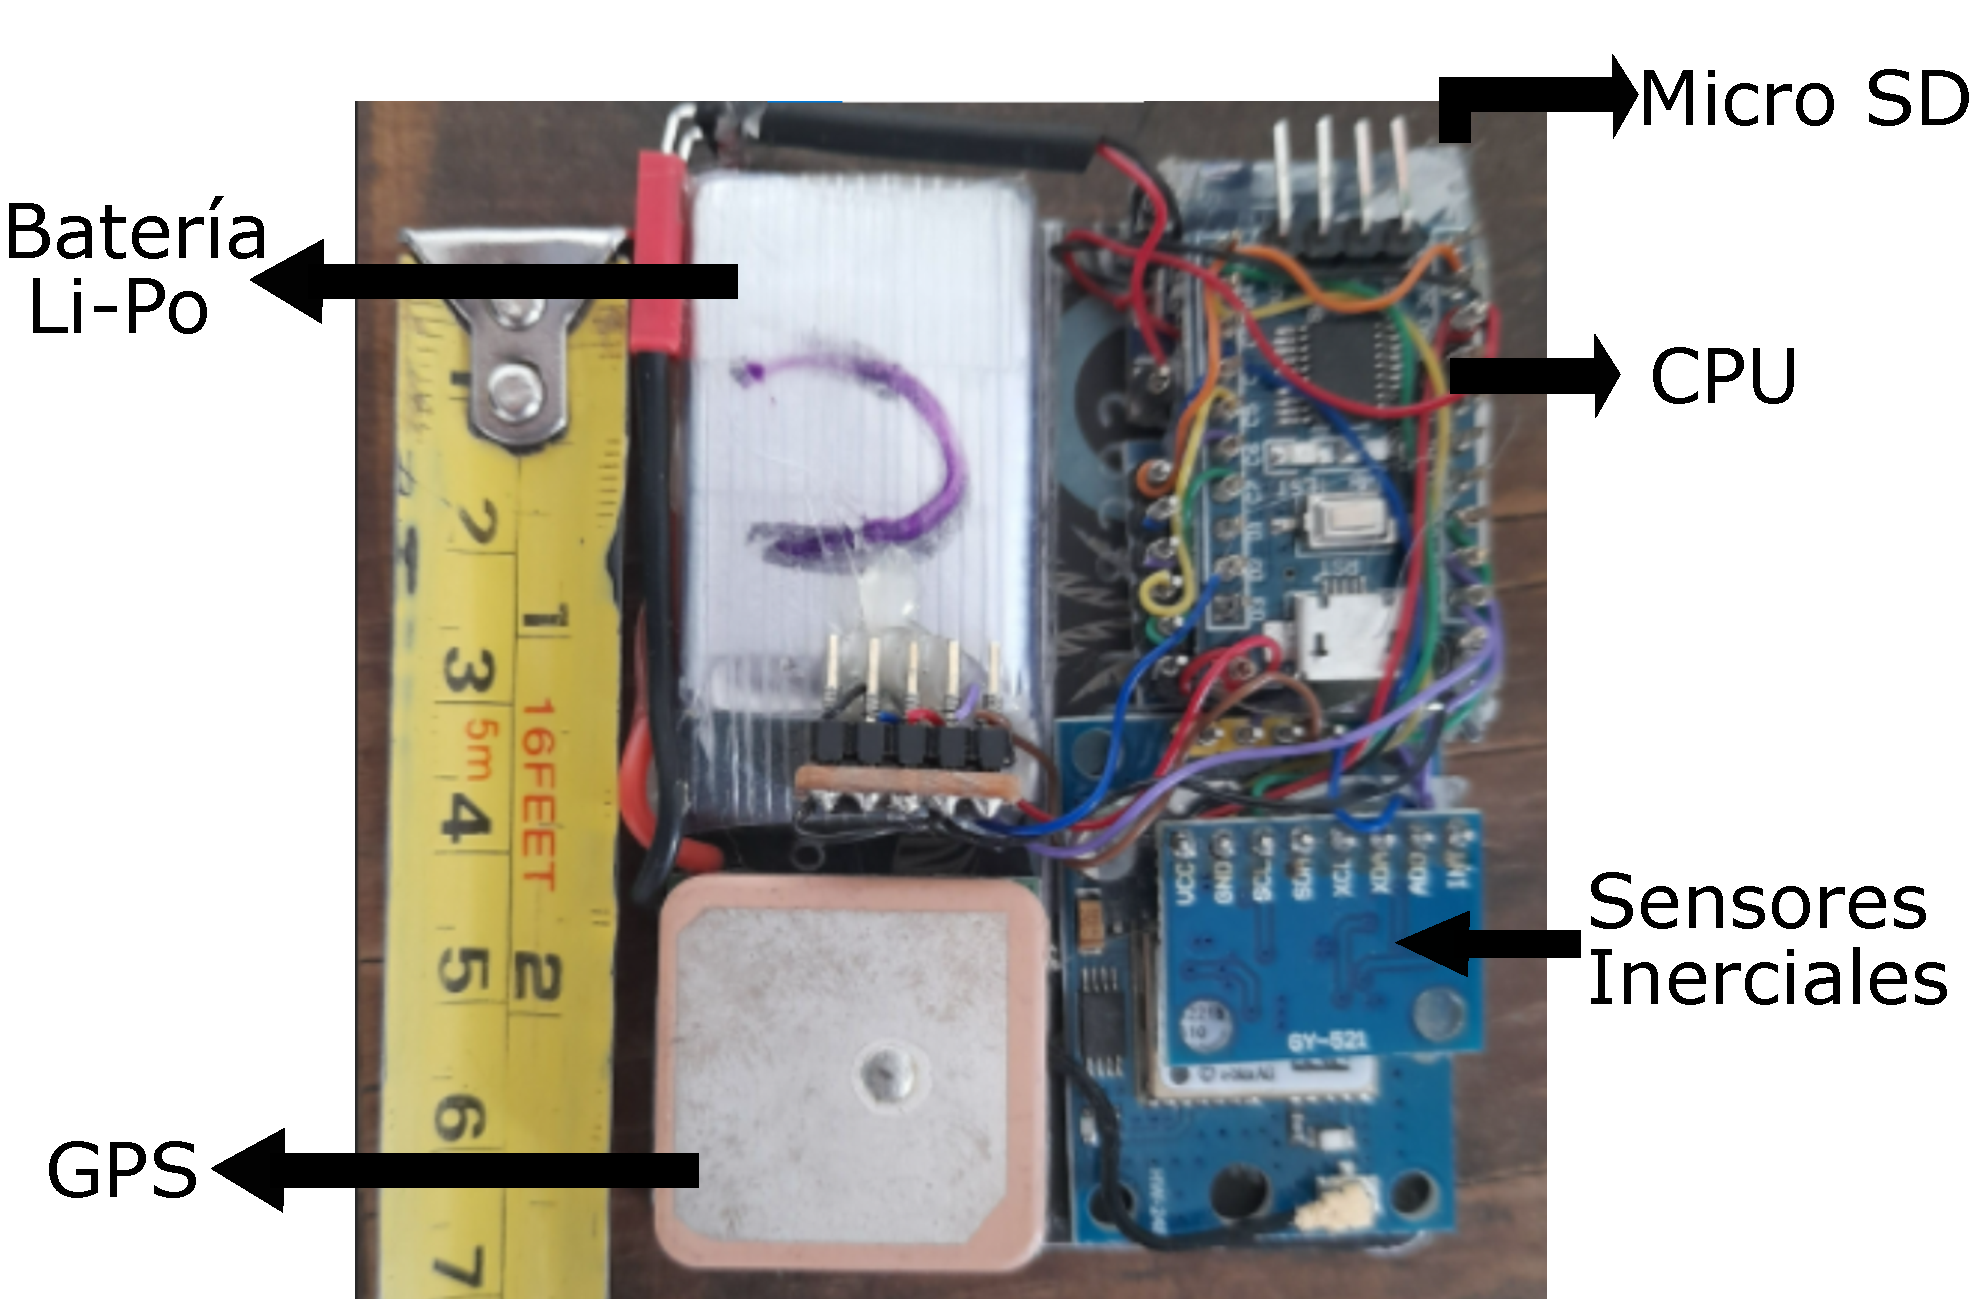
\includegraphics[width=\imsize]{figs/Chap1/tortugometro.pdf}  
\end{center}
    \caption[Unidad de navegación (tortugómetro) para monitorear individuos.] {Unidad de navegación (tortugómetro) para monitorear individuos. Consiste de un GPS, sensores inerciales (giróscopo y acelerómetro) y de temperatura, todos conectados a una unidad de control y procesamiento. Pesa menos de 45g. Las posiciones del GPS son adquiridas cada 10 minutos y se almacenan en la tarjeta micro SD extraíble. }
    \label{fig:tortugometro}
\end{figure}
 
\subsection{i-gotU}
La unidad de navegación comercial i-gotU GT120 (Fig.~\ref{fig:igotu}) es una unidad de bajo costo que permite monitorear la posición de individuos en su hábitat natural. La misma posee un receptor GPS, donde se puede programar la frecuencia de medición a través de un software provisto por el fabricante. La batería de la unidad permite una autonomía de aproximadamente 7 días. El peso de la unidad es de 21 g, lo que representa el 1.5\% del peso de una tortuga de tamaño medio. La unidad  posee una memoria interna que almacena los datos de posición y hora. Los datos se pueden descargar a la computadora a través de un puerto USB.
 
\begin{figure}[ht]
    \begin{center}
       
   
    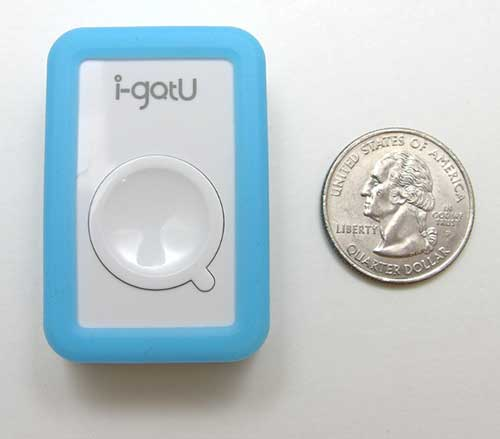
\includegraphics[width=.8\imsize]{figs/Chap1/igotu.jpg}  
\end{center}
    \caption[Unidad de navegación comercial i-gotU para monitorear individuos.] {Unidad de navegación i-gotU para monitorear individuos. Pesa aproximadamente  21\,g, las posiciones del GPS son adquiridas cada 15 minutos y se almacenan en la memoría interna del dispositivo. }
    \label{fig:igotu}
\end{figure}
Con este dispositivo se obtuvieron datos de campañas realizadas entre finales de enero 2022 y abril 2022, se contaron con 12 de estas unidades en correcto funcionamiento y se decidió monitorear a las mismas 6 tortugas intercambiando el i-gotU a cada una de ellas cada 7 días. Se programaron los i-gotU para adquirir posición y hora cada 15 minutos entre las 6 de la mañana y las 9 de la noche, sobre la noche no adquiere datos para ahorrar batería. En total se monitorearon aproximadamente 1000 horas por tortuga ya que algunas semanas no se llegó a intercambiar los i-gotU.
 
\section{Redes complejas}
El uso de herramientas de redes complejas permitió comparar resultados provenientes de diferentes análisis sobre los datos de GPS de las tortugas. En este trabajo se utilizaron métricas sobre la topología de distintas redes generadas, todas calculadas utilizando  funciones implementadas en la librería networkX de Python \cite{networkx}.
 
Una red compleja es un conjunto de elementos (nodos) conectados entre sí por enlaces (aristas). La topología de una red compleja puede ser estudiada a través de distintas métricas. En este trabajo se utilizaron las siguientes métricas:
\begin{itemize}
    \item \textbf{Densidad}: es la fracción de enlaces que existen en la red respecto de la cantidad de enlaces que podrían existir en la red. Se calcula como:
    \begin{equation}
        \rho = \frac{2m}{n(n-1)},
    \end{equation}
    donde $n$ es la cantidad de nodos y $m$ la cantidad de enlaces.
    \item  \textbf{Modularidad}: es una medida de fuerza de división de la red en comunidades. Se calcula como:
    \begin{equation}
        Q = \sum_{c=1}^{n}
        \left[ \frac{L_c}{m} - \gamma\left( \frac{k_c}{2m} \right) ^2 \right]
    \end{equation}
    donde $L_c$ es la cantidad de enlaces que conectan nodos de la comunidad $c$, $k_c$ es la cantidad de enlaces que conectan nodos de la comunidad $c$ con nodos de otras comunidades, $m$ es la cantidad de enlaces en la red y $\gamma$ es un parámetro que depende de la red. En este trabajo se utilizó $\gamma = 1$. Las comunidades en la red se identificaron a través de un método de propagación de etiquetas semi-síncrono \cite{cordasco2010community}.
    \item \textbf{Coeficiente de agrupamiento}: es una medida de la densidad de enlaces entre los vecinos de un nodo. Se calcula como:
    \begin{equation}
        c_u = \frac{2 T(u)}{deg(u)(deg(u)-1)},
    \end{equation}
    donde $T(u)$ es la cantidad de triángulos formados por los vecinos de $u$ y $deg(u)$ es la cantidad de vecinos de $u$ (grado de $u$).
 
   \item \textbf{Centralidad de grado}: para un nodo $v$, la centralidad de grado es la fracción de nodos a la que está conectado. Se calcula como:
    \begin{equation}
        C_G(v) = \frac{deg(v)}{n-1},
    \end{equation}
    donde $deg(v)$ es el grado del nodo $v$ y $n$ es la cantidad de nodos en la red. Da una idea de la importancia relativa de un nodo en la red.
 
\end{itemize}
En los siguientes capítulos se analizarán los datos obtenidos, a través de las metodologías mencionadas, mediante el enfoque de redes complejas.
 
 
 
%%% Local Variables:
%%% mode: latex
%%% TeX-master: "template"
%%% End:
 
 
 
 
 
 


\chapter{Redes de interacción entre tortugas}
\graphicspath{{figs/}}
 
\chapterquote{In retrospect, Euler's unintended message is very simple: Graphs or networks have properties, hidden in their construction, that limit or enhance our ability to do things with them.}{Albert-László Barabási, 1982}
 
\label{Redes de interacción entre tortugas}
\section{Trayectorias }
 
En la Fig.~\ref{fig:trayeSinFiltr} se muestran las trayectorias obtenidas de los datos crudos en el día de medición 1/12/2020. Para graficar el mapa de las trayectorias se realizó un programa en el lenguaje Python utilizando la librería Folium \cite{github}.
 
\begin{figure}[ht]
    \begin{center}
       
   
    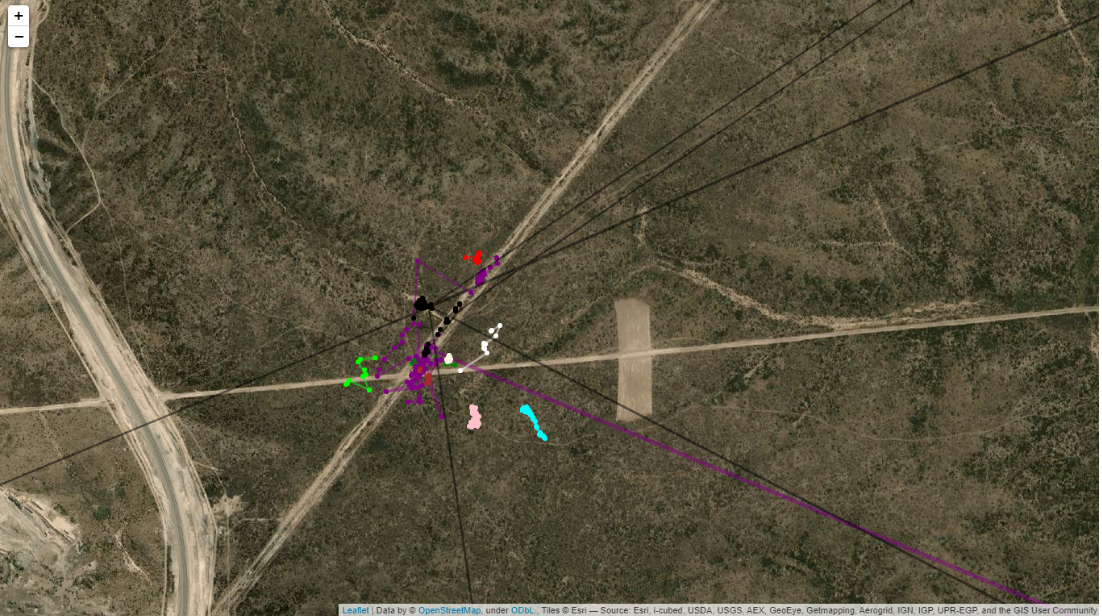
\includegraphics[width=\imsize]{Chap2/Traye1_12_sinF.png}
\end{center}
    \caption[Trayectorias un dia de medición, sin filtrar.]{Trayectorias del 1/12/2020; cada color representa una tortuga diferente. Ambas metodologías fueron implementadas; algunos puntos tomados con el tortugómetro escapan a la trayectoria esperada.}
    \label{fig:trayeSinFiltr}
\end{figure}
Se observa en la Fig.~\ref{fig:trayeSinFiltr}, que algunos puntos tomados por el tortugómetro se desvían de la trayectoria esperada para una tortuga (recorren distancias del orden de los kilómetros en menos de 10 minutos). Se estima que estas desviaciones se producen por dos motivos: en primer lugar, en los primeros minutos de medición, el GPS comienza a conectarse a satélites hasta tener la precisión máxima, haciendo que  los primeros puntos tengan una mayor desviación; en segundo lugar, se observó de manera aleatoria la desviación de algún punto respecto de la trayectoria típica. Para filtrar estas desviaciones, se implementó un método basado en la velocidad máxima que pueden alcanzar los individuos. El mismo está detallado en el repositorio de GitHub, archivo \textit{CriterioParaSacarData.py} \cite{github}. Para obtener la velocidad máxima se calculó la distribución de velocidades de la Fig.~\ref{fig:distribuciondeVel}.
 
 
\begin{figure}[ht]
\begin{center}
       
   
    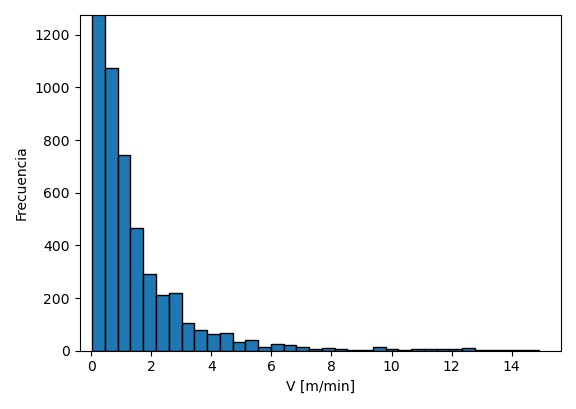
\includegraphics[width=1.2\imsize]{Chap2/Velocidades3.jpeg}
    \caption[Distribución de velocidades.]{Histograma de velocidades en m/min. Las  velocidades obtenidas mayores a 15 m/min están órdenes de magnitud por encima y fueron descartadas.}%re hacer figuras
    \label{fig:distribuciondeVel}
\end{center}
\end{figure}
Se observó en la distribución de velocidades de la Fig.~\ref{fig:distribuciondeVel}, que las tortugas llegan a una velocidad máxima de aproximadamente 15m/min, de manera que se adoptó el criterio de filtrar los tramos de trayectoria en los que la velocidad supera ese valor máximo. Filtrando los puntos de la Fig.~\ref{fig:trayeSinFiltr}, tomando velocidad máxima 15 m/min, se obtuvo  el mapa de la Fig.~\ref{fig:trayeConFiltr}.
 
 
 
 
\begin{figure}[ht]
    \begin{center}
       
   
    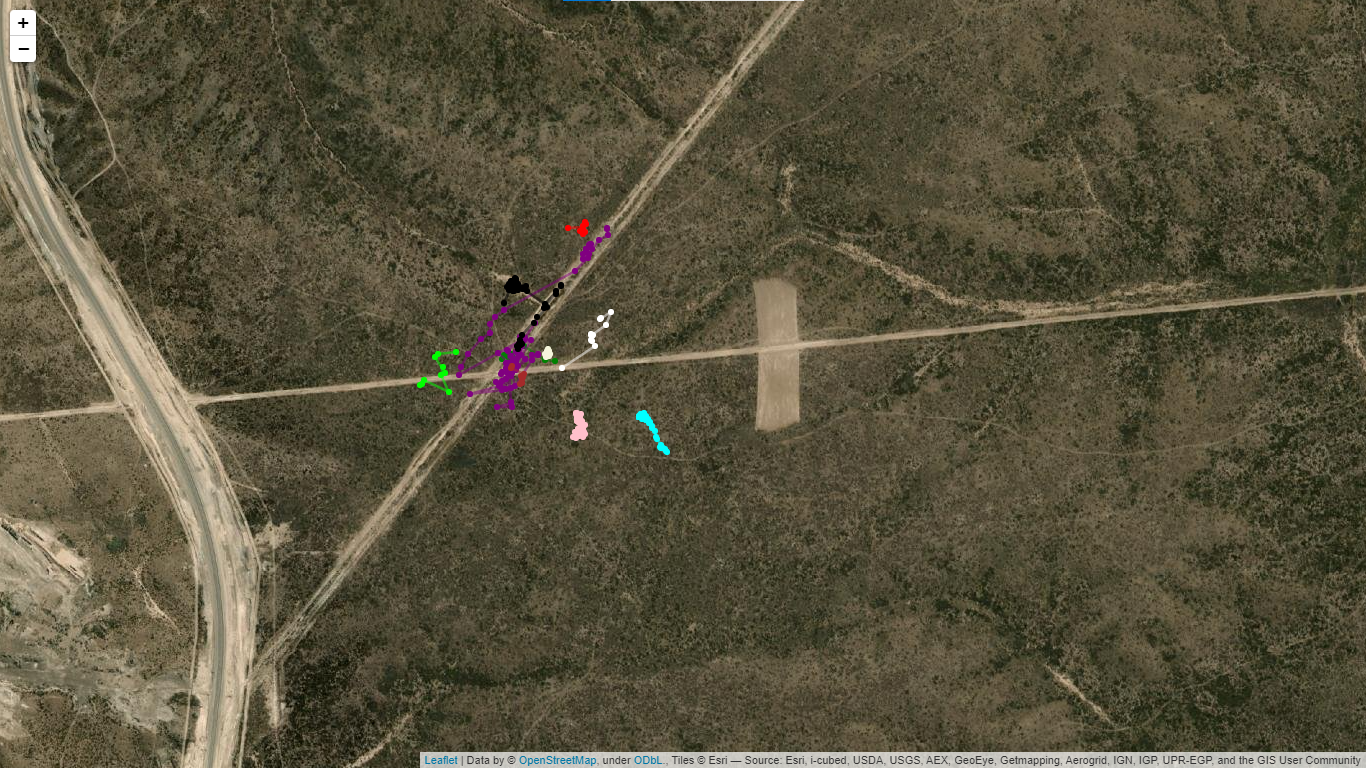
\includegraphics[width=\imsize]{Chap2/Traye1_12_conF.png}
\end{center}
    \caption[Trayectorias un dia de medición, después del filtrado.]{Trayectorias del 1/12/2020 luego del filtrado; cada color representa una tortuga diferente.}
    \label{fig:trayeConFiltr}
\end{figure}
 
\section{Zonas de interés}
Partiendo de las trayectorias filtradas, se realizó  una grilla identificando las zonas de recurrencia en la Fig.~\ref{fig:grilla1}. Las celdas de la grilla fueron elegidas de 10\,m$^2$ debido a que se estima en 10\,m el erorr del GPS del tortugómetro. Para cada celda se contó el numero de veces que estuvo allí, la grilla fue programada en Python \cite{github}. En caso de que se pudieran identificar los factores o características de las zonas más recurridas, se podrían sugerir políticas de manejo para minimizar los daños sobre las tortugas. Esto es especialmente importante dado que ahora se está introduciendo ganado en la zona con el consiguiente deterioro del hábitat natural de las mismas.
 
 
\begin{figure}[ht]
    \begin{center}
    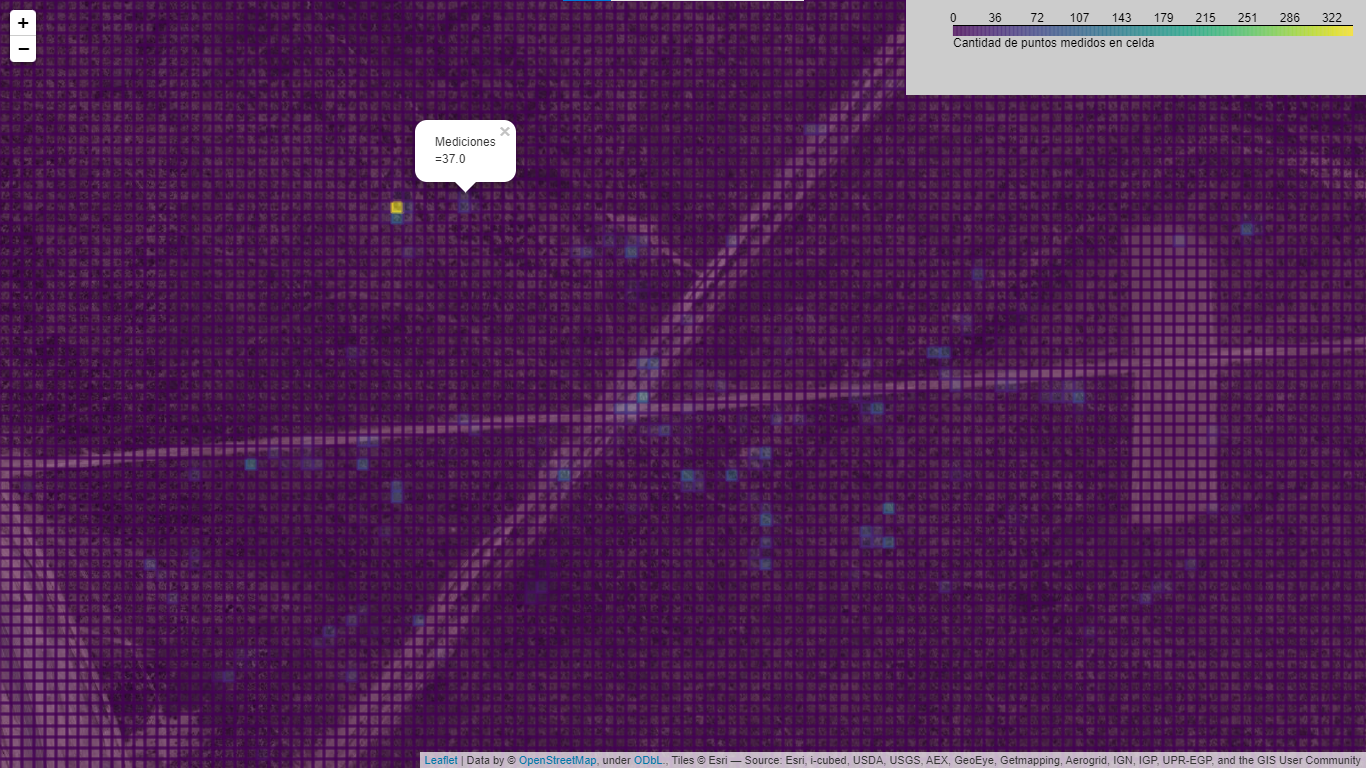
\includegraphics[width=\imsize]{Chap2/GrillaSintCNoche.png}
    \end{center}
    \caption[Mapa de zonas de recurrencia.]{Mapa de recurrencias  interactivo con las trayectorias filtradas. Al hacer clic en cualquier celda de la grilla un cartel dice cuantas mediciones fueron tomadas. El tamaño de celda es de 10m$^2$.}
    \label{fig:grilla1}
\end{figure}
 
Se puede observar en la Fig.~\ref{fig:grilla1} un punto que se destaca mucho más que el resto (arriba a la izquierda) teniendo el máximo de mediciones en esa casilla. Esto se debe a que una pareja de tortugas pasó la noche con el tortugómetro puesto en medio de un arbusto de difícil acceso. Para obtener una mejor idea de las zonas de interés diurnas se realizó otra grilla usando sólo datos del tortugómetro registrados en el día (entre 7am y 9pm) y  realizando una interpolación lineal de 1 punto por minuto por cada par de puntos consecutivos (Fig.~\ref{fig:grillaInt}, \cite{github}). Esta interpolación da una aproximación de las casillas por donde tuvo que pasar la tortuga y añade un peso cuando la tortuga se quedó dentro de la misma casilla por una mayor cantidad de tiempo (mediciones consecutivas).
 
\begin{figure}[ht]
    \begin{center}
       
   
    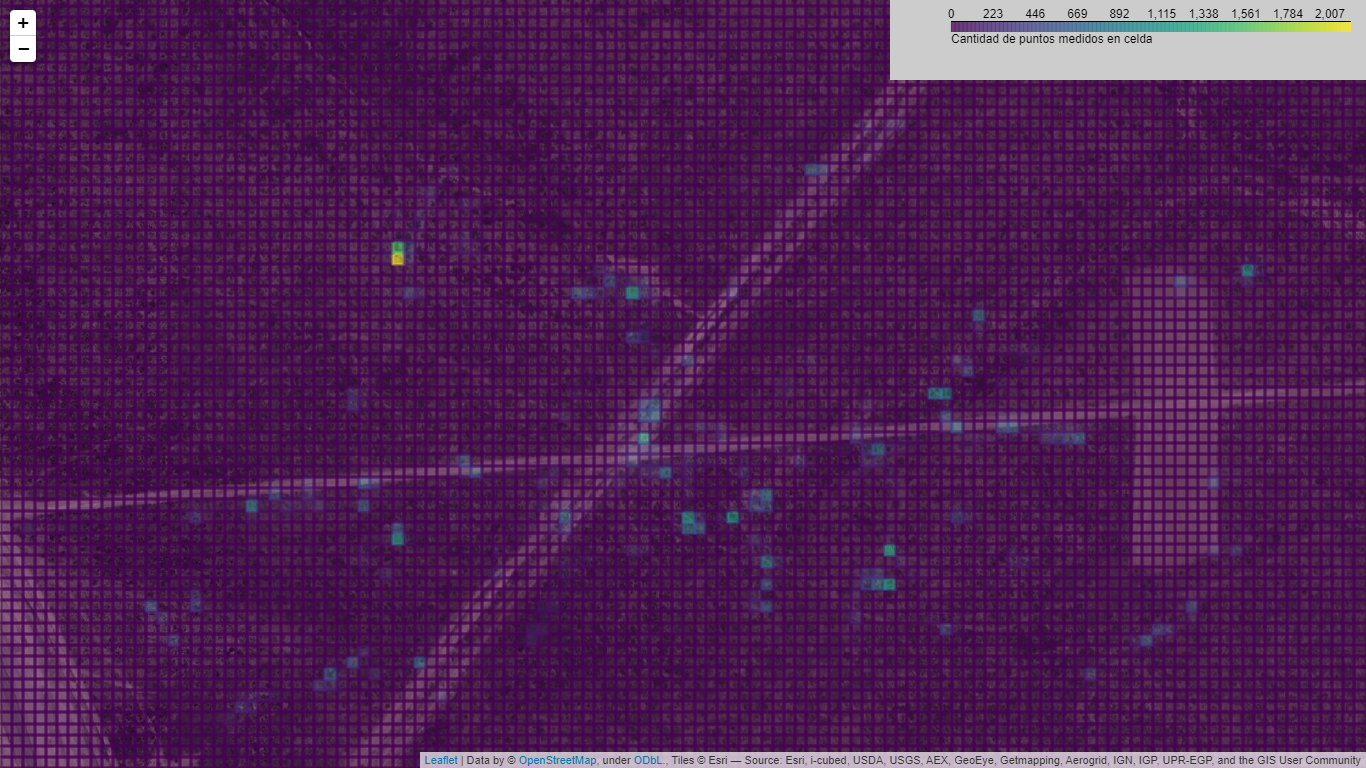
\includegraphics[width=\imsize]{Chap2/GrillaCintSNoche.png}
\end{center}
    \caption[Mapa con zona de recurrencia para trayectorias diurnas.]{Mapa de recurrencias  interactivo con las trayectorias diurnas (7am-9pm) filtradas e interpoladas linealmente. Al hacer clic en cualquier celda de la grilla un cartel dice cuantas mediciones fueron tomadas. El tamaño de celda es de 10m$^2$.}
    \label{fig:grillaInt}
\end{figure}


Comparando las Figs. \ref{fig:grilla1} y \ref{fig:grilla1}, se observa en la  Fig.~\ref{fig:grillaInt} un mayor contraste de las otras celdas respecto al que se encuentra arriba a la izquierda. Esto se debe a la extracción de los puntos nocturnos. Al momento se desconocen los motivos por los cuales dichas zonas son muy visitadas, esto será investigado en profundidad en el futuro.
 
\section{Red de encuentros}
Partiendo de las trayectorias filtradas, se decidió buscar el solapamiento de las trayectorias, para identificar los encuentros. Para ello, se implementó un código en Python que, partiendo de cualquier punto de su trayectoria, busca si hay otro punto de otra tortuga que se encuentre a una distancia menor a 20 metros y a una distancia temporal menor a 20 minutos. Cuando se cumple esta condición se van guardando los pares de puntos junto con la hora y el nombre de ambas tortugas.
 
En las Figs. \ref{fig:encuentros_hora_medida_tortugometro} y \ref{fig:encuentros_hora_medida_igotu}, pueden verse la cantidad de encuentros calculados por hora medida por los tortugómetros y por los i-gotU en función de los meses de medición. Los encuentros del tipo macho-hembra fueron normalizados por la cantidad promedio de horas medidas de ambos sexos para cada mes, en cambio para la cantidad de encuentros macho-macho y hembra-hembra se normalizó utilizando la cantidad de horas medidas para cada sexo en cada mes.  
\begin{figure}[ht]
    \begin{center}
       
   
    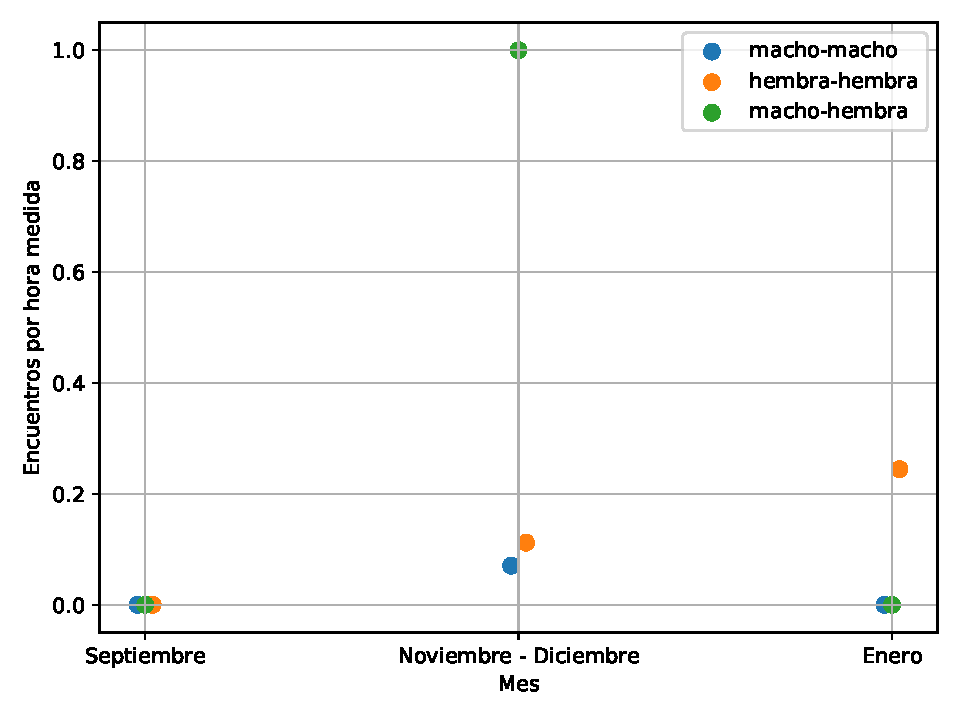
\includegraphics[width=\imsize]{Chap2/encuentros_por_hora_tortugometro.pdf}
\end{center}
    \caption[Encuentros por hora medida tomando los datos del tortugómetro.]{Encuentros sobre cantidad de horas medidas para cada sexo en función de los meses de medición utilizando el tortugómetro. Los distintos colores identifican el tipo de encuentro.}
    \label{fig:encuentros_hora_medida_tortugometro}
\end{figure}
 
\begin{figure}[ht]
    \begin{center}
       
   
    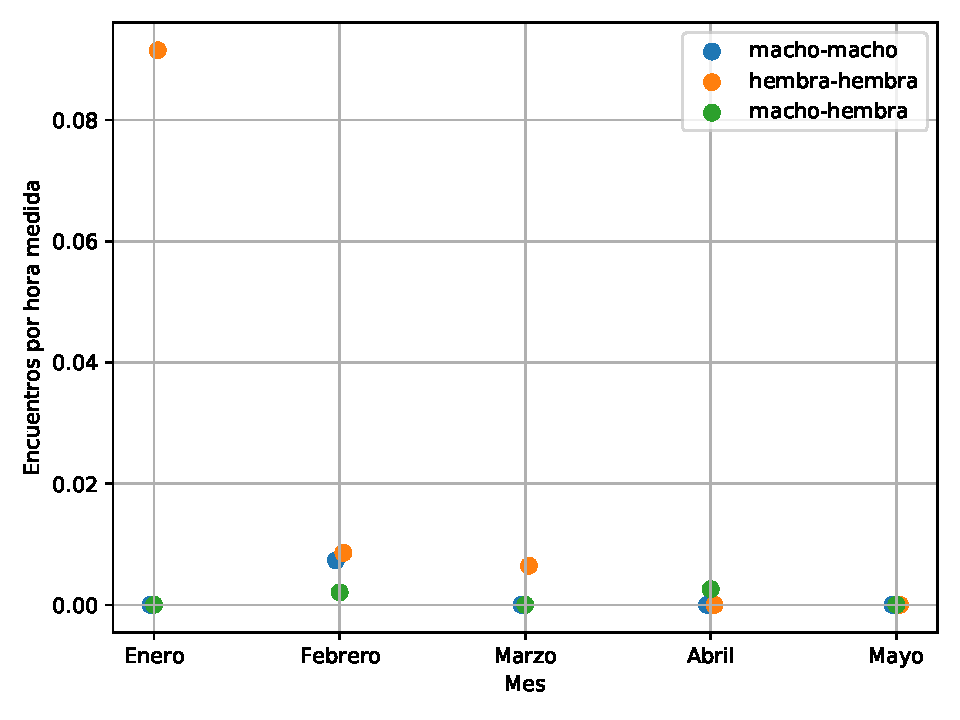
\includegraphics[width=\imsize]{Chap2/encuentros_por_hora_igotu.pdf}
\end{center}
    \caption[Encuentros por hora medida tomando los datos de los i-gotU.]{Encuentros sobre cantidad de horas medidas para cada sexo en función de los meses de medición utilizando los i-gotU. Los distintos colores identifican el tipo de encuentro.}
    \label{fig:encuentros_hora_medida_igotu}
\end{figure}
En la Fig. \ref{fig:encuentros_hora_medida_tortugometro}, se observa que el máximo de encuentros del tipo macho-hembra por hora medida ocurre en los meses noviembre-diciembre; esto coincide con la época de apareamiento. Estos meses están juntos ya que las mediciones en esos meses fueron tomadas a finales de noviembre y principios de diciembre. Para el mes de enero solo se registraron encuentros del tipo hembra-hembra en ambas figuras ( \ref{fig:encuentros_hora_medida_tortugometro} y \ref{fig:encuentros_hora_medida_igotu}), esto puede deberse a que las hembras están buscando un lugar acorde para depositar sus huevos, haciendo el encuentro hembra-hembra más probable. Para los datos de los i-gotU (\ref{fig:encuentros_hora_medida_igotu}) también se registraron encuentros en los meses de febrero, marzo y abril, pero en menor cantidad que en los meses anteriores, asociamos esta diferencia a la disminución de actividad en las tortugas propia de este periodo.
 
 
Utilizando los encuentros calculados, se armaron dos redes de interacción  utilizando la librería NetworkX \cite{networkx}, una para los datos obtenidos con  tortugómetro y otra para los datos provenientes de i-gotU (Figs. \ref{fig:redInteraccion20mincampanas} y \ref{fig:redInteraccion20igotu}). Las conexiones entre nodos tortugas tienen peso linealmente dependiente de la cantidad de encuentros entre ellas, esto se observa en el grosor del link entre dos tortugas y las distancias relativas entre nodos.
 
 
\begin{figure}[ht]
    \begin{center}
       
   
    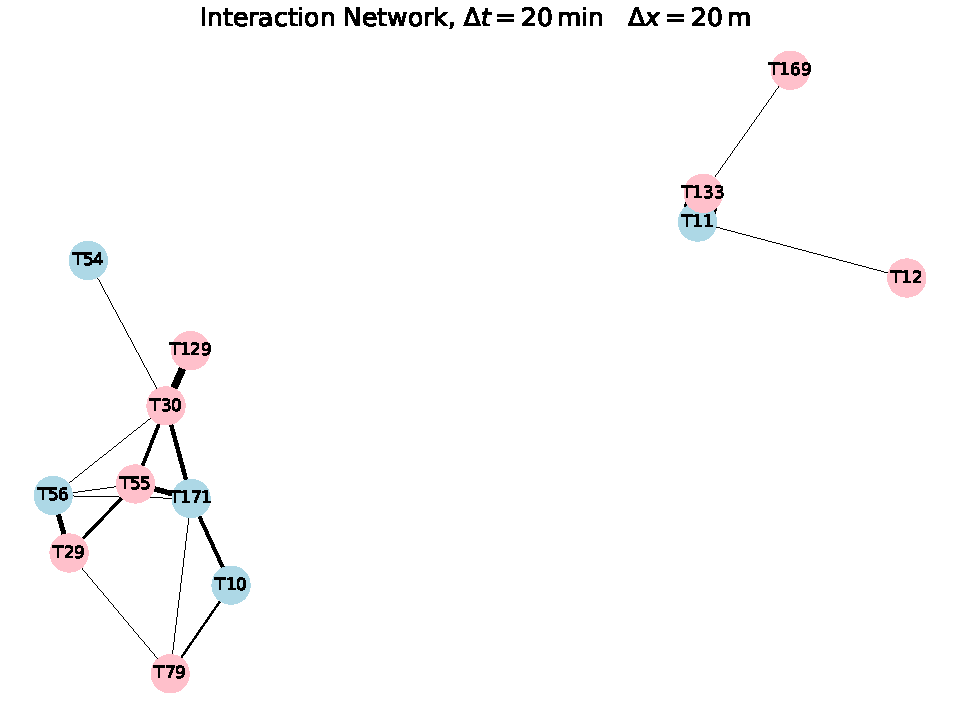
\includegraphics[width=\imsize]{Chap2/red_interaccion_20min_campanas.pdf}
\end{center}
    \caption[Red de encuentros entre tortugas  con datos tomados por el tortugómetro.]{Red de encuentros entre tortugas para datos provenientes de la metodología  tortugómetro. La condición de encuentro está dada por una distancia espacial menor a 20 metros y a una distancia temporal menor a 20 minutos. Los datos de tortugómetros fueron tomados en distintas campañas en los meses de octubre, noviembre, diciembre y mediados de enero.}
    \label{fig:redInteraccion20mincampanas}
\end{figure}
 
 
 
\begin{figure}[ht]
    \begin{center}
       
   
    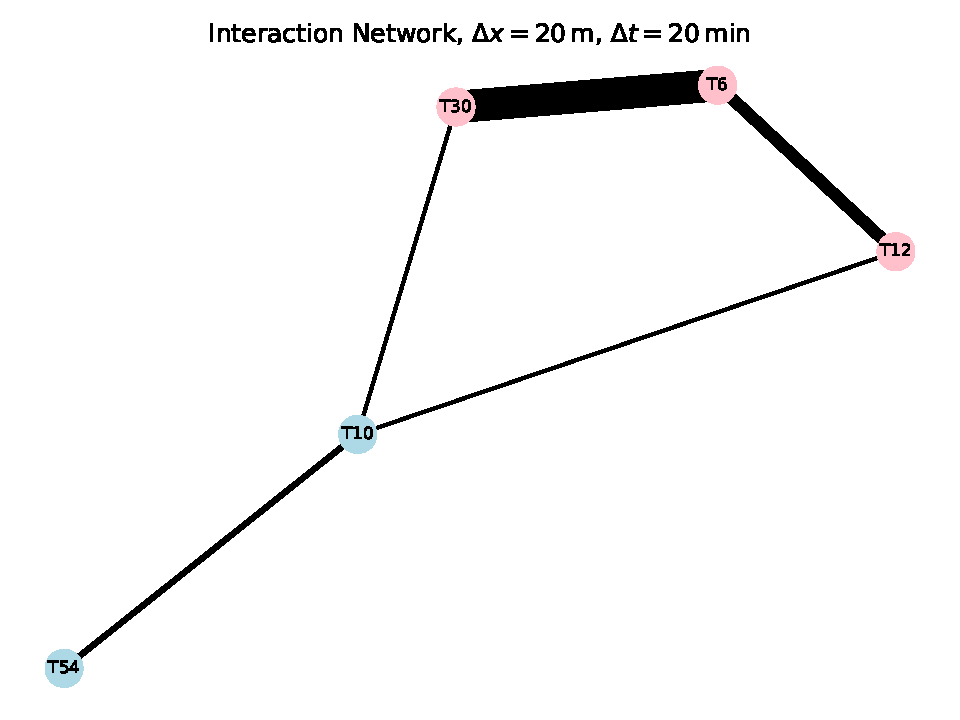
\includegraphics[width=\imsize]{Chap2/red_interaccion_20min_IGOTO.pdf}
\end{center}
    \caption[Red de encuentros entre tortugas utilizando i-gotU.]{Red de encuentros entre tortugas para datos provenientes de las metodologías i-gotU. La condición de encuentro está dada por una distancia espacial menor a 20 metros y a una distancia temporal menor a 20 minutos. Los datos de los i-gotU fueron tomados desde finales de febrero hasta principios de mayo.}
    \label{fig:redInteraccion20igotu}
\end{figure}
 
 
En la Fig. \ref{fig:redInteraccion20mincampanas}, se observa que la red de interacción está compuesta por dos comunidades. Sobre estas comunidades, se calcularon la media de las posiciones de cada nodo tortuga junto con su desviación estándar y no se encontraron diferencias significativas en estos valores para  nodos tortugas pertenecientes a cada una de las comunidades. Esto nos indica que las tortugas que pertenecen a cada comunidad, no están separadas en el espacio y no es la causa de la separación de la red en dos comunidades. Queda a determinar en futuros trabajos si la separación de la red en estas dos comunidades está relacionada con la cantidad de  mediciones o con alguna característica de la población de tortugas estudiada. En la red, también se observan diferencias  de grado, teniendo algunas tortugas muchas más conexiones que otras. Se seguirá trabajando para identificar comportamientos particulares de las tortugas que puedan estar relacionados con la distribución de grado de la red.
 
En la Fig. \ref{fig:redInteraccion20igotu}, se observa una mayor cantidad de encuentros entre las tortugas hembras (grosor de enlace), esto puede deberse a la época de medición, ya que en enero las tortugas hembras están en búsqueda de algún lugar para depositar sus huevos. En el siguiente capítulo se analizarán redes bipartitas de refugios y se compararan con las redes de interacción de tortugas para entender mejor este aspecto.
 
%%% Local Variables:
%%% mode: latex
%%% TeX-master: "template"
%%% End:
 
 
 


\chapter{Uso de refugios}
Para varias especies los refugios son fundamentales para la protección de predadores y  condiciones climáticas (especialmente para animales de sangre fría, como las tortugas). En especies relativamente solitarias, los individuos pasan un tiempo considerable solos en los refugios y tienen pocos encuentros directos fuera de la época de apareamiento.
Ejemplos de estas especies incluyen a los mapaches, zorros rojos, orangutanes y algunas especies de abejas, avispas y murciélagos. Para estas poblaciones de animales salvajes, monitorear y entender estos refugios puede ayudar a establecer patrones sociales de los individuos.
 
En distintos campos cercanos a la zona de medición (San Antonio Oeste, provincia de Río Negro) estan introduciendo ganado al habitad de las tortugas, es importante entender si presenta una amenaza para la integridad de los refugios y entender el patron de movimiento  de las tortugas sobre los mismos, junto con las caracteristicas geograficas de los refugios mas usados.
 
\section{Refugios en el mapa}
Para determinar el refugio donde pasó la noche la tortuga se tomaron dos criterios, uno para cada una de las metodologías de medición en los sets de datos. Para el tortugometro se tomó el último punto tomado de la tortuga en un día de medición y se pidió la condición de que haya sido tomado después de las 20 horas, en base a las anotaciones tomadas por el grupo, las tortugas generalmente  se encontraban en el refugio cuando quitaban los tortugometros después de este horario. A este punto nuevo se le asigna un label de refugio y un enlace con la tortuga que pasó la noche en ese refugio. A medida que se añade otro refugio primero se verifica que presente una distancia mayor a 20 metros con todos los otros refugios etiquetados, en caso que la distancia sea menor a 20 metros a por ejemplo el refugio 1, se dice que la tortuga estuvo en el refugio 1.
 
Para los datos tomados por los i-gotU, se decidió mirar primero las distancias entre el último punto medido (21 horas) de algún día monitoreado con el primer punto del día siguiente (6 horas). Y también se miraron las distancias entre el primer punto de algún día de monitoreo con el segundo punto (6 horas y 6:15 respectivamente). En la Fig. \ref{fig:distancias} se muestran los histogramas de las distancias entre los puntos. Se observa que entre el último punto de la noche y el primero de la mañana distancias mayores a 20 metros son muy probables con varias mediciones de distancias del orden de los 50 o 100 metros, lo que nos diría que la tortuga todavía no se encuentra en el refugio a esa hora (21 horas). En cambio, entre el primer punto del día y el segundo punto, las distancias menores a 20 metros son las más probables, lo que nos diría que la tortuga todavía no abandonó el refugio entre las 6 y las 6:15, a excepción de algunos pocos casos donde tenemos distancias del orden de los 50 m. Por eso para los datos de los i-gotU se decidió tomar el primer punto del día como la posición del refugio y se siguió el mismo procedimiento de los tortugometos para agregar labels a los refugios. De cara a las próximas campañas se decidió mantener las mediciones del i-gotU entre las 21 y las 6 horas, pero disminuyendo la frecuencia de muestreo.
 
 
\begin{figure}[ht]
    \begin{center}
        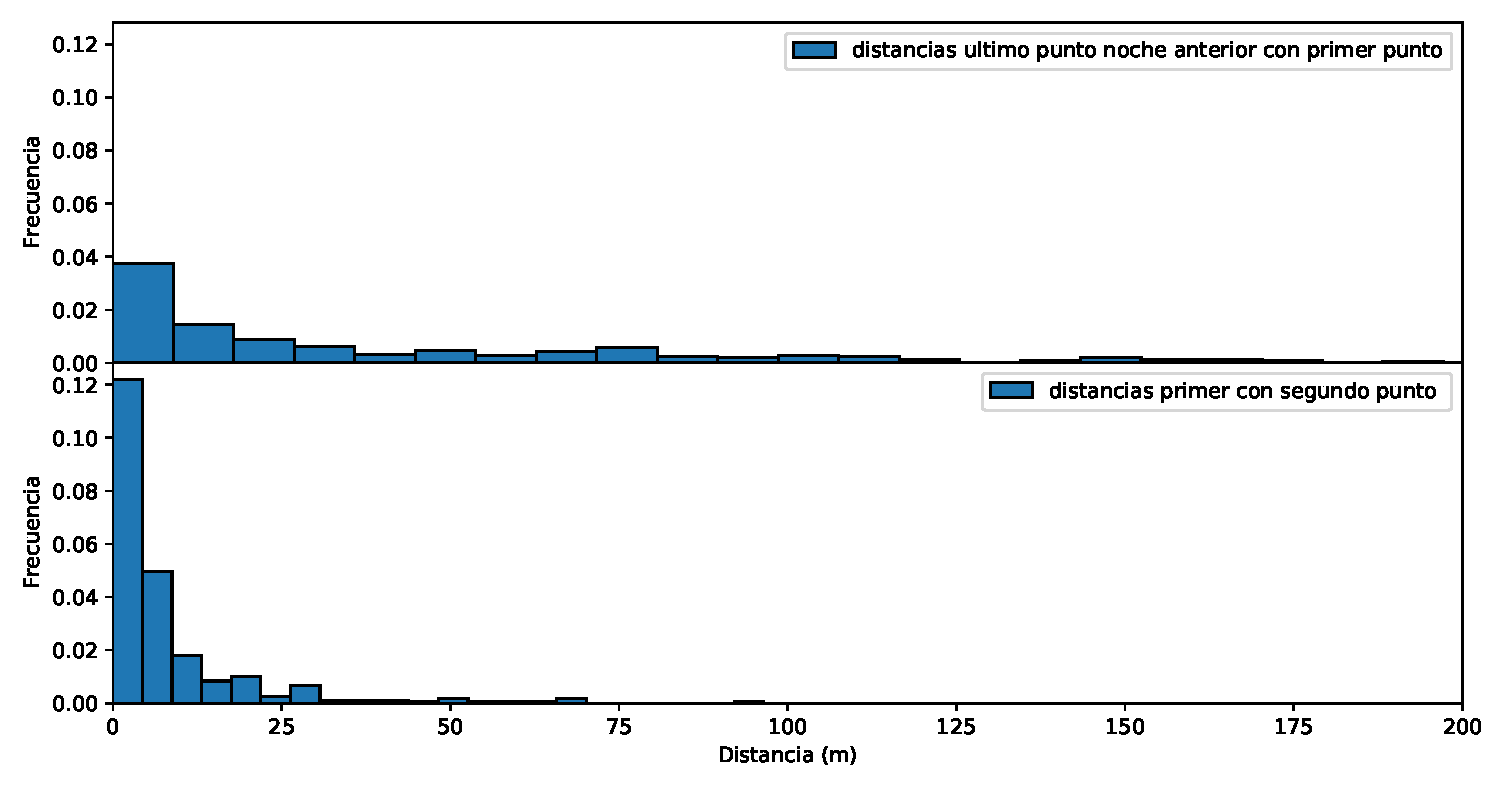
\includegraphics[width=1.4\imsize]{Chap3/Distancias_primer_ult_con_deteterminar_criterio_ref.pdf}
        \caption[Histogramas de las distancias entre los puntos de los datos de i-gotU.]{ Histogramas de las distancias entre los puntos de los datos de i-gotU. Arriba se muestra la distancia entre el último punto del día anterior y el primer punto del día siguiente. Abajo se muestra la distancia entre el primer punto del día y el segundo punto del día.}
        \label{fig:distancias}
        \end{center}
\end{figure}
 
Se graficaron los refugios encontrados en un mapa utilizando la librería Folium, los mapas fueron guardados en formato html para el fácil acceso a los mismos, al clickear en un refugio sobre el html aparece un cartel con las tortugas que pasaron la noche en el refugio. En las Fig. \ref{fig:refus_campanas_con_labels} y \ref{fig:refus_igotu_labels} se muestran los mapas de los refugios encontrados para los datos de las campañas y los datos de i-gotU respectivamente.
 
 
\begin{figure}[ht]
    \begin{center}
        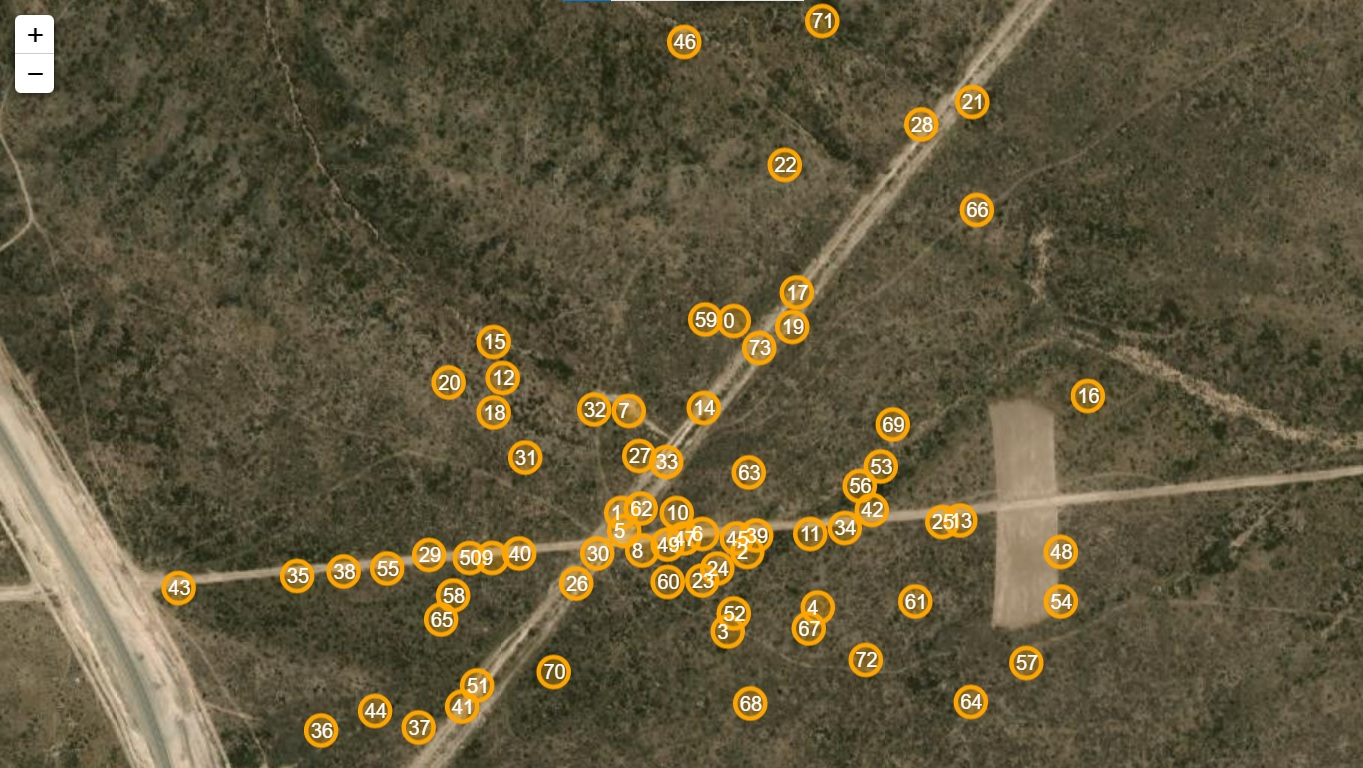
\includegraphics[width=\imsize]{Chap3/map_refugies_with_labels.jpg}
        \caption{Distribución geográfica de los refugios encontrados para los datos provenientes de las campañas.}
        \label{fig:refus_campanas_con_labels}
       
        \end{center}
\end{figure}
 
\begin{figure}[ht]
    \begin{center}
        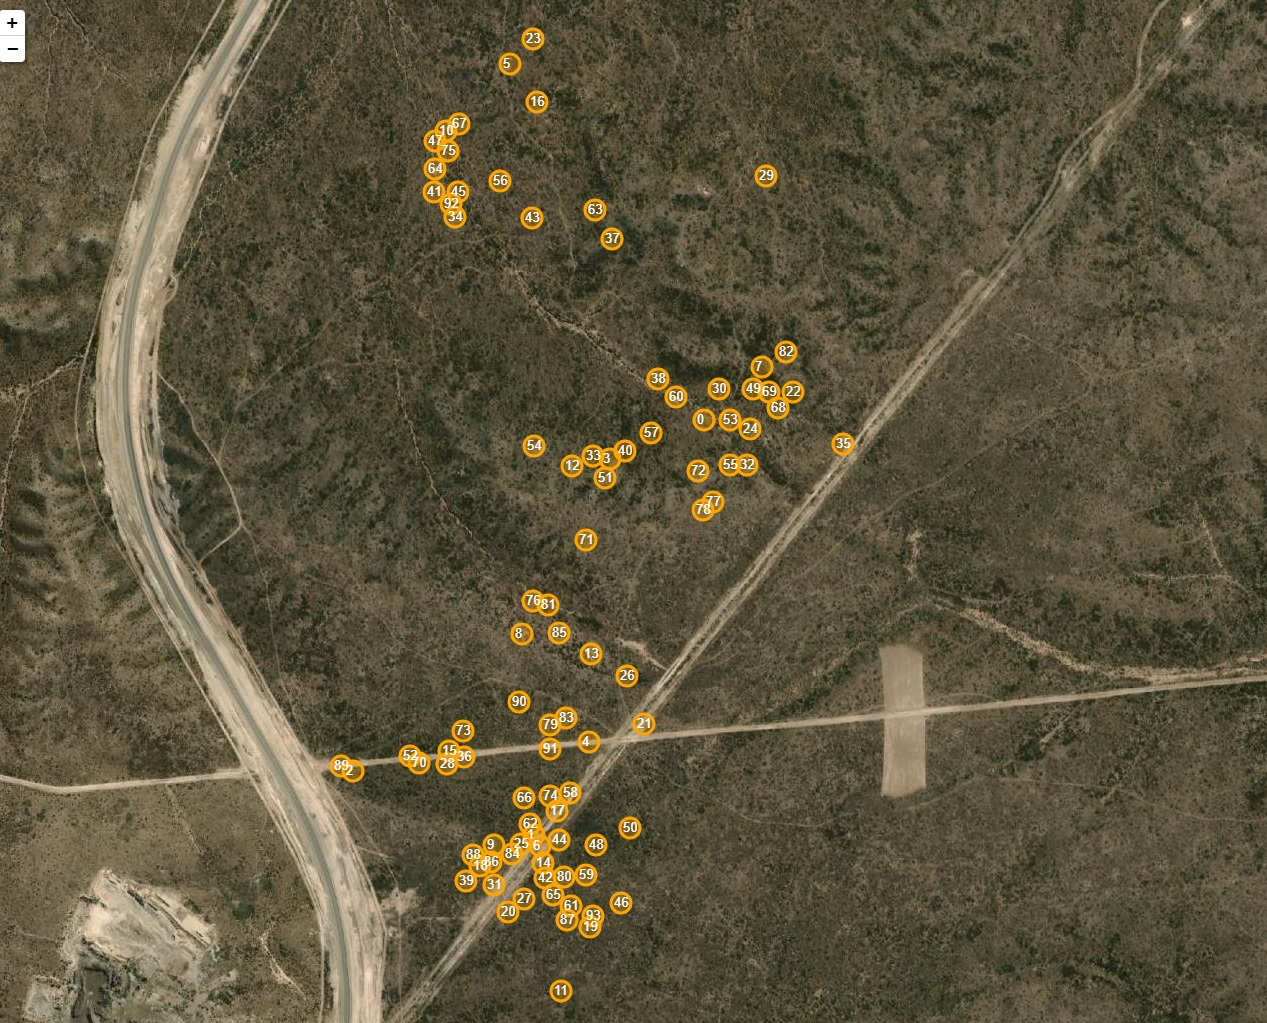
\includegraphics[width=\imsize]{Chap3/map_refugies_with_labels_IGOTo.jpg}
        \caption{Distribución geográfica de los refugios encontrados para los datos provenientes de los datos de i-gotU.}
        \label{fig:refus_igotu_labels}
       
        \end{center}
\end{figure}
 
En base a observaciones de directas de campo \cite{Erika}, se espera que las tortugas machos tengan una distribución de refugios más amplia en el espacio que las hembras.  Para verificar esta hipótesis se definieron dos métricas, centro de masa de refugios y distancia media entre refugios. El centro de masa se define como:
\begin{center}
   
 
$$X_{centro}= \sum^{N -1}_{n=0} \frac{i_{n} X_n}{I_{totales}}.$$
\end{center}
Donde $I_{totales}$ es la cantidad de noches donde se registró que la tortuga durmió en un refugio (depende de cada tortuga), $X_n$ es la coordenada X del refugio n, $i_{n}$ es la cantidad de noches que la tortuga durmió en el refugio n y N la cantidad de refugios totales.  Este proceso se calcula para todas las tortugas.
Partiendo de $X_{centro}$, la distancia media  espacial de los refugios se calcula como:
$$D = \sum^{N -1}_{n=0} \frac{|X_n i_n - X_{centro}|}{I_{totales}}.$$
\label{eq:distancia_media_refugios}
Esta métrica fue calculada para todas las tortugas y  promediada para  machos y hembras. Se encontró para los machos $\overline{D}_m =  (128\pm66)\,\text{m}$ y para las hembras     $\overline{D}_h = (122\pm82)\,\text{m}$. Es decir que no se encontraron diferencias significativas en la distribución espacial de refugios  entre machos y hembras.
\section{Refugios más usados y caminos tomados}
Dentro de los refugios que utiliza una tortuga, se encontraron refugios preferidos, es decir refugios que fueron visitados recurrentemente. Para observar esto se decidió graficar la acumulada de noches pasadas en un refugio para los refugios más utilizados por una tortuga. Esto se realizó solo para los datos provenientes de los i-gotU, ya que se contó con una gran cantidad de días consecutivos de medición. En la Fig. \ref{fig:refugios_preferidos} se encuentra la acumulada de noches pasadas en estos refugios que distintas tortugas tomaron como preferidos.
 
\begin{figure}[ht]
    \begin{center}
        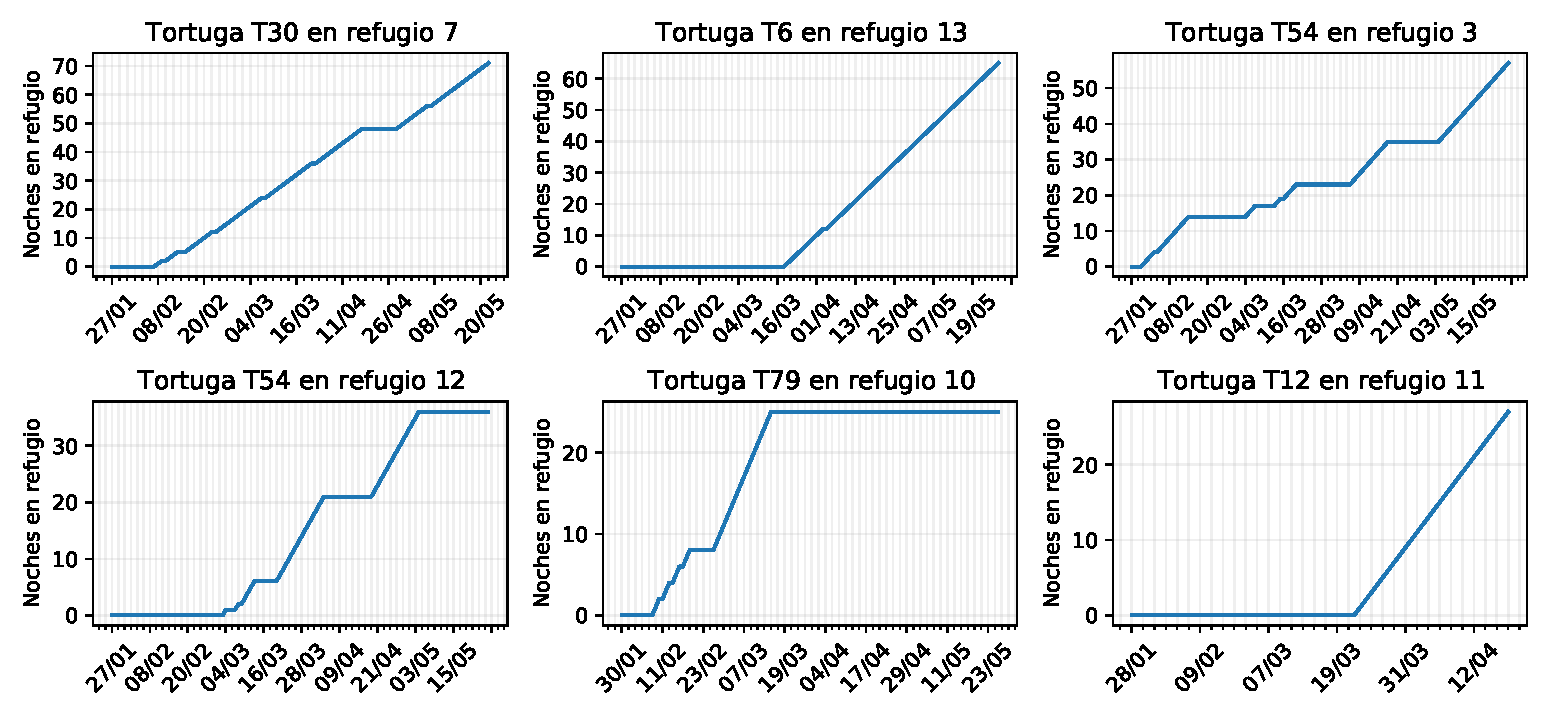
\includegraphics[width=1.4\imsize]{Chap3/acumulada_de_noches_en_refmasUsados_espanol.pdf}
        \caption[Acumulada de noches pasadas en los refugios preferidos.]{Acumulada de noches pasadas en los refugios preferidos para distintas tortugas monitoreadas por los i-gotU de enero 2022 a mayo 2022.}
        \label{fig:refugios_preferidos}
       
        \end{center}
\end{figure}
Se observa en la Fig. \ref{fig:refugios_preferidos} que las tortugas tienen un refugio como preferido donde pasan la mayor parte de las noches monitoreadas. Sin embargo, también se observó que algunas tortugas tienen varios refugios preferidos, como es el caso de la tortuga T54. En las tortugas T30, T54, T6 y T79, se registraron días donde decidió pasar la noche en otro refugio para después volver a su refugio preferido. Para visualizar estas rutas entre refugios y la preferencia relativa entre ciertos refugios, se realizaron mapas en la librería Folium donde se graficaron los refugios con tamaños proporcional a la cantidad de noches que la tortuga pasó en el refugio con conexiones entre refugios ilustrando las rutas tomadas entre refugios. Es decir si la T54 pasó una noche en el refugio 12 y la noche siguiente en el refugio 3, hay una línea entre el refugio 12 y el refugio 3 en el mapa. En la Fig. \ref{fig:ruta_refus_T54} se muestra un ejemplo de este tipo de mapa para la tortuga T54.
 
\begin{figure}[ht]
    \begin{center}
        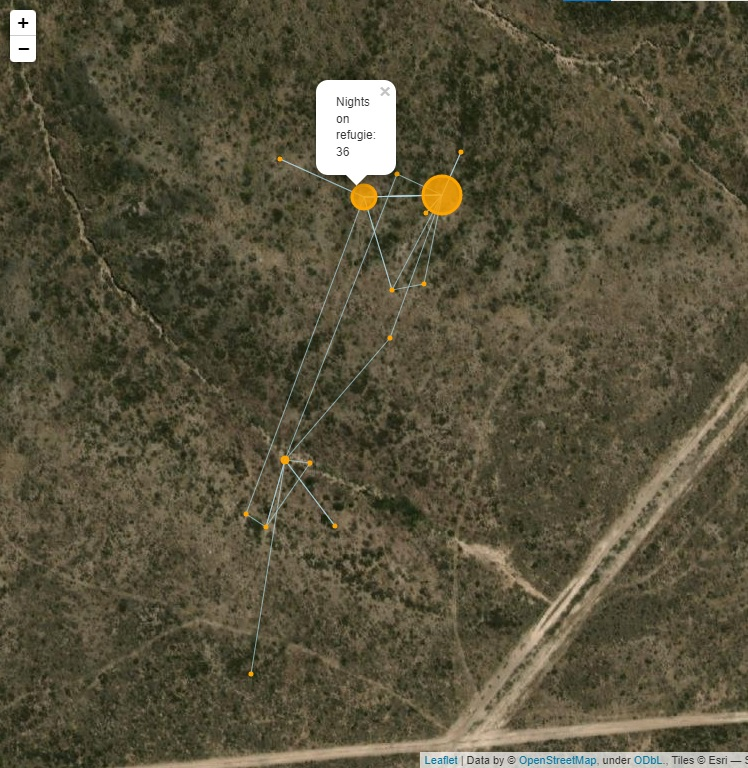
\includegraphics[width=\imsize]{Chap3/refugies_path_for_t54.jpg}
        \caption[Caminos tomados entre refugios para la tortuga T54.]{Caminos tomados entre refugios para la tortuga T54. El tamaño de nodo refugio es proporcional a la cantidad de noches que pasó la tortuga en el mismo. Una conexión entre par de nodos refugios aparece solo si pasó una noche en el refugio de origen y la noche siguiente en el refugio de destino. Al clickear sobre un nodo refugio se puede ver la cantidad de noches que pasó la tortuga en el mismo.}
        \label{fig:ruta_refus_T54}
       
        \end{center}
\end{figure}
Haber encontrado preferencia por ciertos refugios abre distintas preguntas, ¿Qué características comparten estos refugios preferidos? ¿Siguen recurriendo estos refugios a distintas épocas del año u otros años?  Responder estas preguntas podría ayudarnos a plantear medidas de conservación de la especie. En futuras campañas de medición se espera poder entender más sobre estos refugios preferidos.
 
 
 
 
\section{Redes  de bipartitas de refugios}
Se armaron redes bipartitas con nodos refugios y nodos tortugas. Los nodos refugios solo están conectados con nodos tortugas.  Partiendo de todos los labels de refugios con las tortugas que pasaron noche en ese refugio se armaron las redes bipartitas para los datos tomados por los tortugometros y los datos tomados con los i-gotU, Figs. \ref{fig:red_bipartita_refus_campanas} y \ref{fig:red_bipartita_refus_igotu} respectivamente.
 
\begin{figure}[ht]
    \begin{center}
        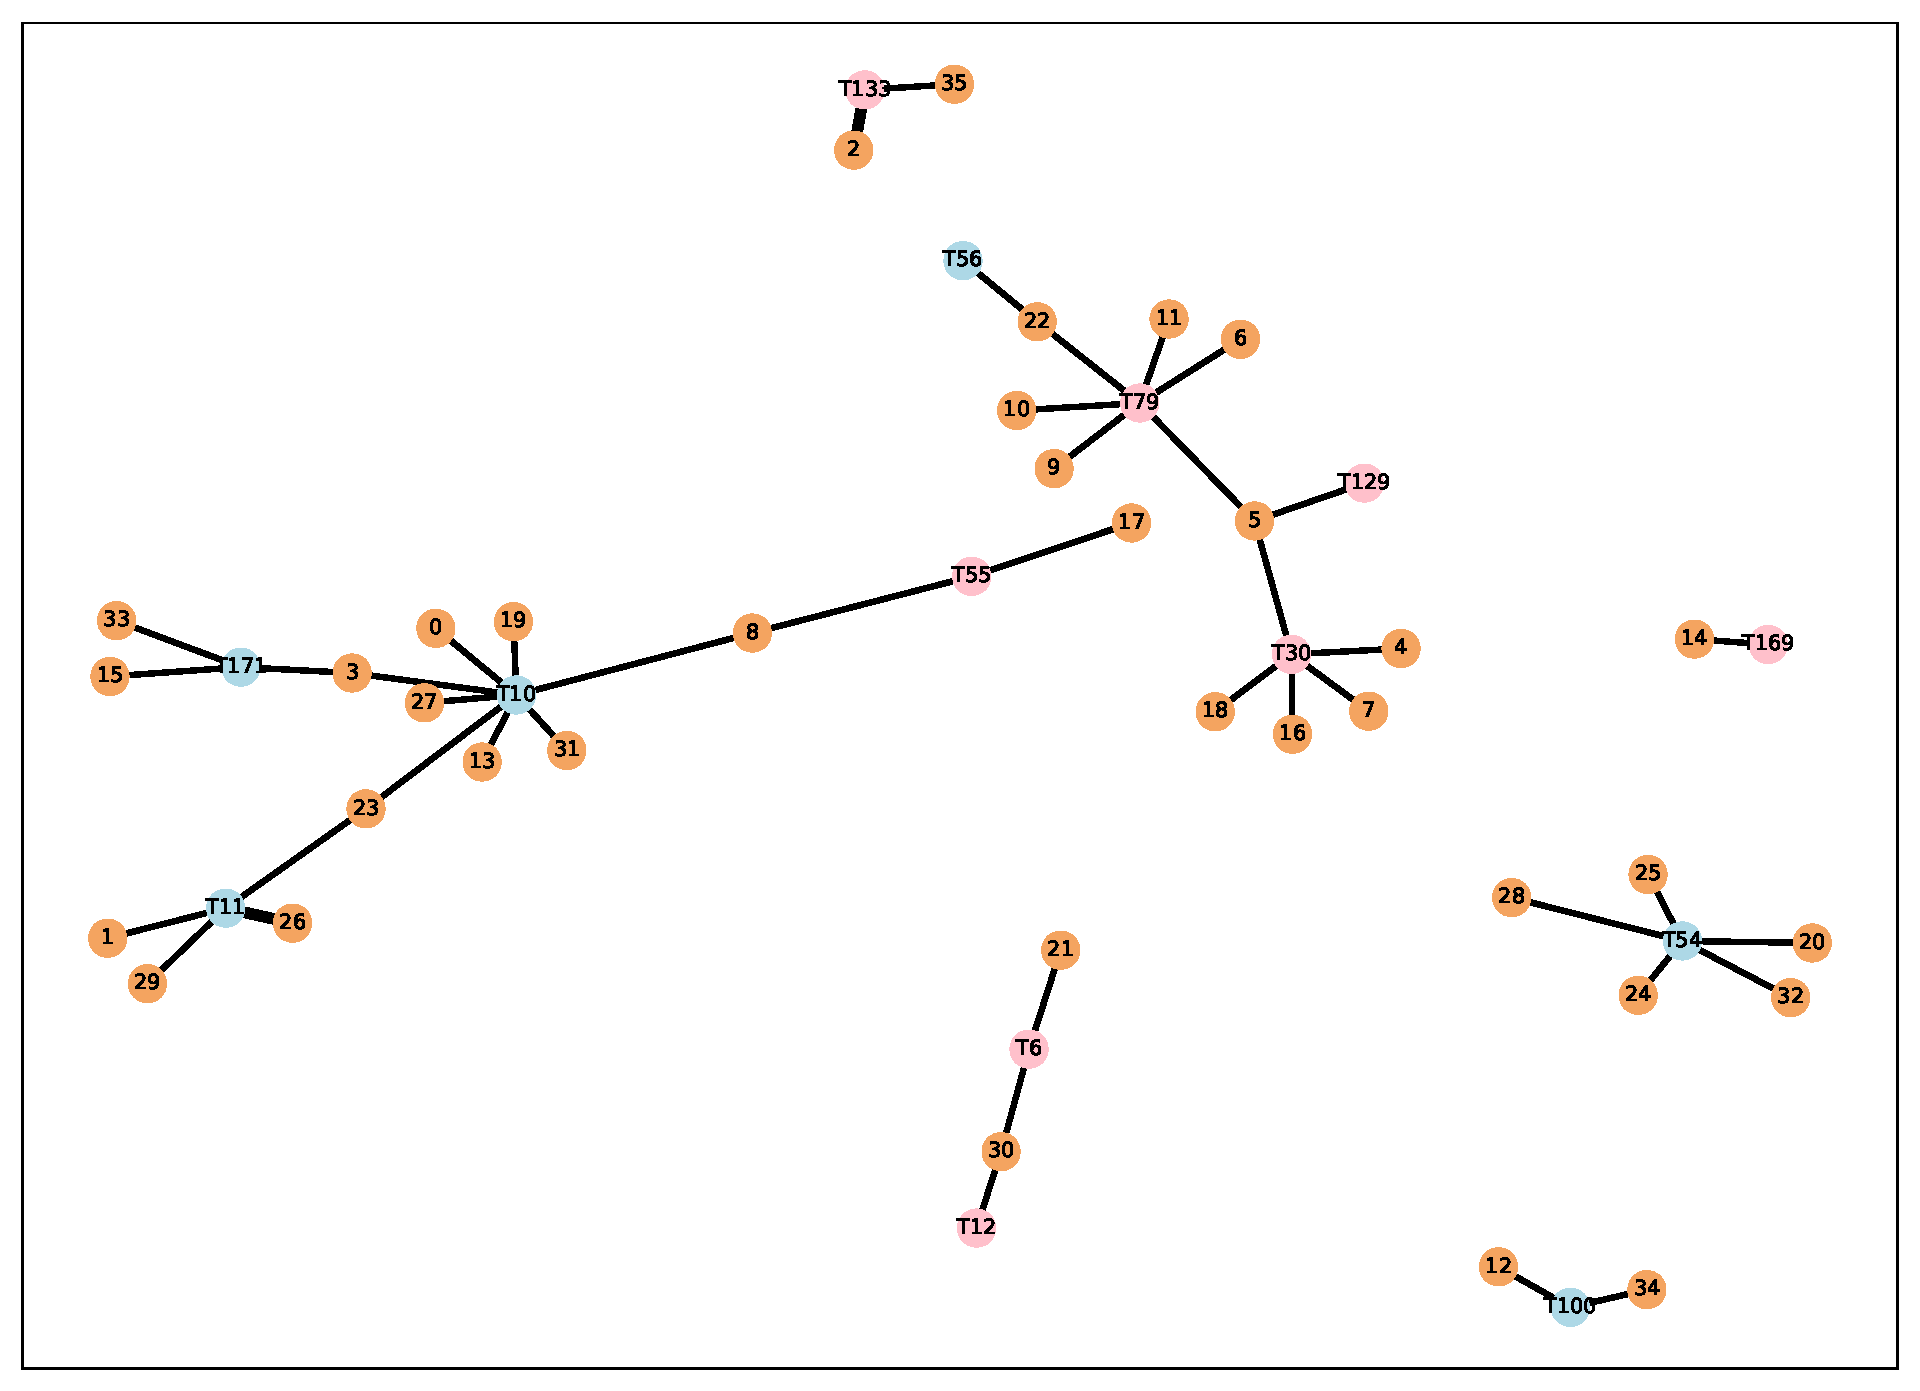
\includegraphics[width=\imsize]{Chap3/RedBipartita_deRefugios_corregida_campanas_2300.pdf}
        \caption[Red bipartita de refugios para los datos de los tortugometros.]{Red bipartita de refugios para los datos de los tortugometros. Las distancias relativas entre nodos y el grosor del link son dependientes de la cantidad de noches que una  tortuga paso en el refugio. }
        \label{fig:red_bipartita_refus_campanas}
       
        \end{center}
\end{figure}
 
\begin{figure}[ht]
    \begin{center}
        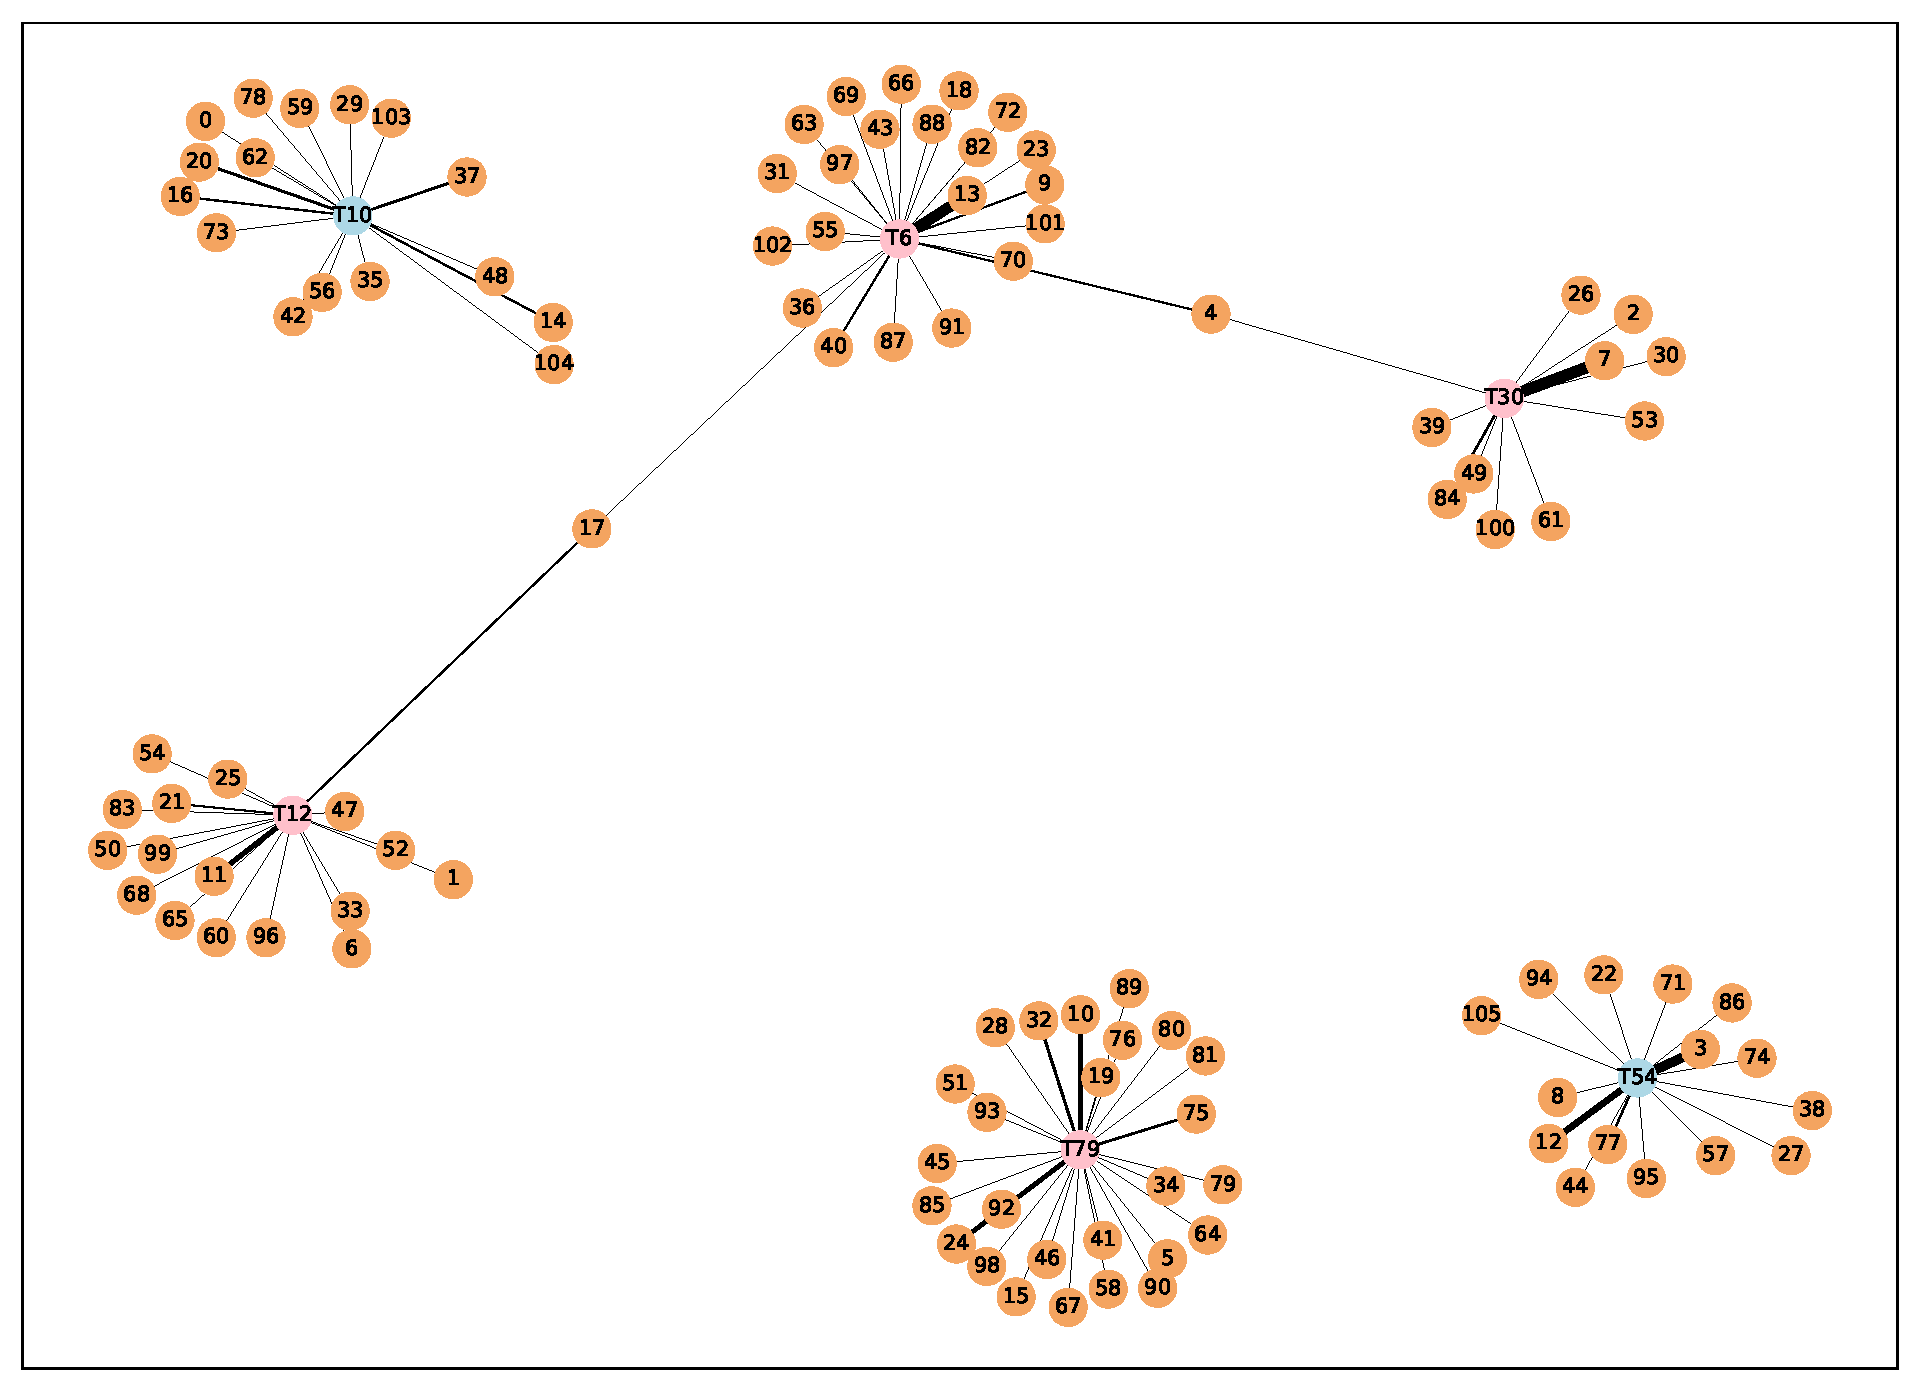
\includegraphics[width=1.3\imsize]{Chap3/RedBipartita_deRefugios_IGOTO.pdf}
        \caption[Red bipartita de refugios para los datos de los i-gotU.]{Red bipartita de refugios para los datos de los i-gotU. Las distancias relativas entre nodos y el grosor del link son dependientes de la cantidad de noches que una  tortuga paso en el refugio. }
        \label{fig:red_bipartita_refus_igotu}
       
        \end{center}
\end{figure}
En la Figs. \ref{fig:red_bipartita_refus_campanas} y \ref{fig:red_bipartita_refus_igotu}, se observan refugios compartidos entre dos y tres pares de refugios.  En base a este resultado, se decidió buscar la probabilidad de que dos nodos tortugas estén conectados en la red de encuentros (Figs. \ref{fig:redInteraccion20mincampanas} y \ref{fig:redInteraccion20igotu}). Al proyectar la red bipartita en nodos tortugas obtenemos una redes comparables con las redes de encuentros, en las Figs. \ref{fig:proyeccion_red_campanas} y \ref{fig:proyeccion_red_igotu}.
 
 
\begin{figure}[ht]
    \begin{center}
        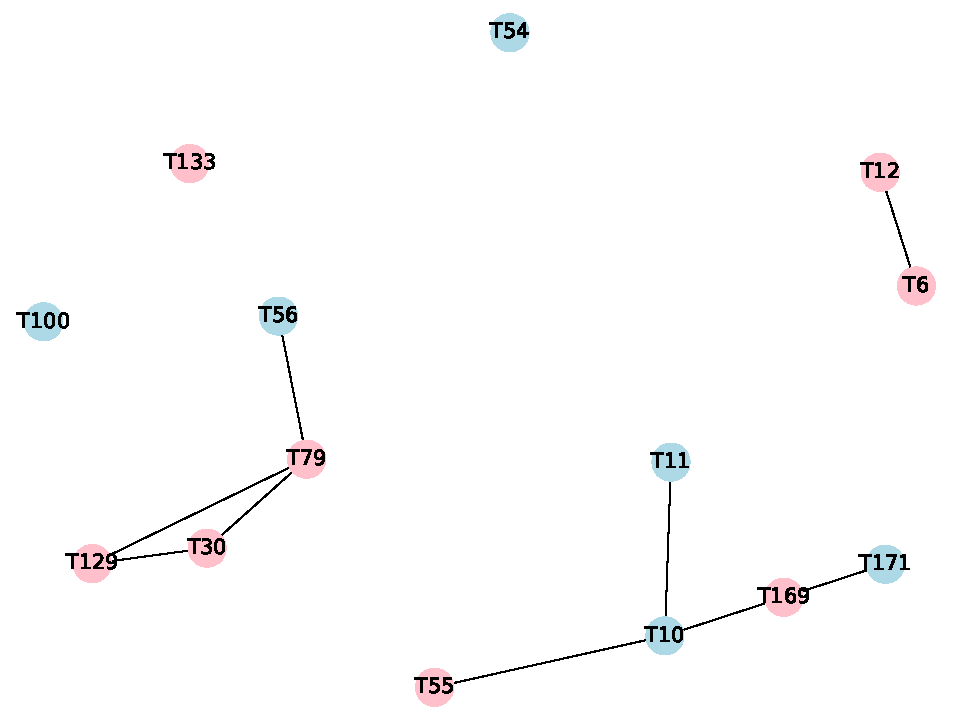
\includegraphics[width=\imsize]{Chap3/Proyecion_bipartita_ref_solo_tortus.pdf}
        \caption[Proyección  de red bipartita de refugios para datos de los tortugometros en nodos tortugas.]{Proyección  de red bipartita de refugios para datos de los tortugometros (Fig. \ref{fig:red_bipartita_refus_campanas}) en nodos tortugas. Si hay una refugio compartido por un par de nodos tortugas, aparece una conexión entre este par de nodos en la proyección. }
        \label{fig:proyeccion_red_campanas}
       
        \end{center}
\end{figure}
 
\begin{figure}[ht]
    \begin{center}
        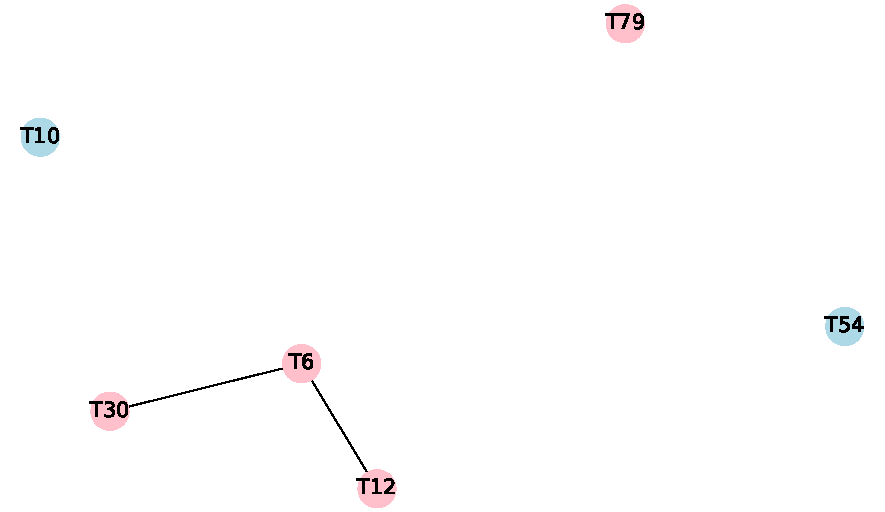
\includegraphics[width=\imsize]{Chap3/Proyecion_bipartita_ref_solo_tortus_IGOTU.pdf}
        \caption[Proyección  de red bipartita de refugios para datos de los tortugometros en nodos tortugas.]{Proyección  de red bipartita de refugios para datos de los i-gotU (Fig. \ref{fig:red_bipartita_refus_igotu}) en nodos tortugas. Si hay una refugio compartido por un par de nodos tortugas, aparece una conexión entre este par de nodos en la proyección. }
        \label{fig:proyeccion_red_igotu}
       
        \end{center}
\end{figure}
Para comparar y ver que tan probable es el encuentro entre tortugas en caso que hayan usado alguna vez el mismo refugio, se decidió tomar las proyecciones de las redes bipartitas como predictores de conexiones en las redes de encuentros. Se calcularon las métricas precisión, accuracy y recall, partiendo de las cantidades TP, TN, FP y FN. Donde, por ejemplo, TP se calculó como la cantidad de conexiones existentes en las redes de encuentros que están en las redes proyectadas. Los valores obtenidos se muestran el la tabla \ref{tab:metricas_comparacion_redes}.
\begin{table}[ht]
    \centering
    \begin{tabular}{|c|c|c|c|}
       
   \hline
    Metodología  & precision & Recall & accuracy \\ \hline
    Tortugometro & 0.125     & 0.059  & 0.258    \\ \hline
    i-gotU       & 1         & 0.4    & 0.4       \\ \hline
   
    \end{tabular}
    \caption[Tabla con métricas de comparación entre redes de encuentros y proyecciones de redes bipartitas.]{Tabla con métricas de comparación entre redes de encuentros y proyecciones de redes bipartitas. Se tomó las proyecciones de la redes bipartitas como predictor de conexiones en las redes de encuentros.}
    \label{tab:metricas_comparacion_redes}
\end{table}
Se observa en la tabla \ref{tab:metricas_comparacion_redes}, que las métricas obtenidas para los datos provenientes de los tortugometros son considerablemente menores que las métricas obtenidas para los datos provenientes de los i-gotU. Estas diferencias se espera que estén asociadas a la poca cantidad de refugios nocturnos medidos para los datos del tortugometro ya que originalmente las campañas de medición no se planearon para este tipo de análisis. Por otro lado, con los i-gotU se monitorean una menor cantidad de tortugas, haciendo posible la existencia de un bias de medición.
 
Para determinar si los resultados de la tabla \ref{tab:metricas_comparacion_redes} son estadísticamente significativos, se realizaron operaciones de \textit{double edge swap} sobre las redes bipartitas de refugios y se compararon los valores obtenidos sobre estas nuevas redes generadas, después de las proyecciones. Se realizó un código en Python que elige dos conexiones al azar en la red bipartita y las intercambia si es que no existe ya estas conexiones. Es decir, si T10 uso el refugio 54 y T11 el refugio 32, se intercambian los enlaces en caso que T10 no tenga una conexión con el refugio 32 y tampoco la T11 con el 54 \cite{github}, este procedimiento se itera de manera de generar una red aleatoria manteniendo la distribución de grado constante (un equivalente en cierto sentido a mantener la misma cantidad de mediciones pero tomando uso de refugios al azar). Partiendo de 1000 redes generadas a partir de 1000 cambios aleatorios de conexiones (1000 \textit{double edge swap}), se obtuvieron las métricas de precisión, recall y accuracy para cada red generada. Sobre estos valores se calculó la cantidad de veces donde las métricas halladas por usos aleatorios de refugios fueron mayores que los valores obtenidos para los datos de la tabla \ref{tab:metricas_comparacion_redes}. Los resultados se muestran en la tabla \ref{tab:metricas_comparacion_redes_aleatorias}.
\begin{table}[ht]
    \centering
    \begin{tabular}{|c|c|c|c|}
       
   \hline
    Metodología  & \% Precisión mayor  &  \% Recall mayor & \% Accuracy mayor \\ \hline
    Tortugometro & 60    & 50  & 50    \\ \hline
    i-gotU       & 0        & 0    & 0      \\ \hline
   
    \end{tabular}
    \caption[Tabla con comparación de métricas obtenidas en redes bipartitas con usos aleatorios de refugios respecto a las métricas medidas.]{Tabla con comparación de métricas obtenidas por redes bipartitas con usos aleatorios de refugios respecto a las métricas medidas. Se tomó las proyecciones de la redes bipartitas generadas aleatoriamente como predictor de conexiones en las redes de encuentros y se calcularon las proporciones donde estas métricas son mayores a las obtenidas por la tabla \ref{tab:metricas_comparacion_redes}.}
    \label{tab:metricas_comparacion_redes_aleatorias}
\end{table}
Se observa en la tabla \ref{tab:metricas_comparacion_redes_aleatorias}, que las métricas obtenidas para los datos provenientes de los i-gotU son estadísticamente significativas, mientras que las métricas obtenidas para los datos provenientes de los tortugometros no lo son. Esto se debe a que la cantidad de refugios nocturnos medidos para los datos del tortugometro es considerablemente menor que la cantidad de refugios nocturnos medidos para los datos de los i-gotU. Por otro lado, con los i-gotU se monitorean una menor cantidad de tortugas, haciendo posible la existencia de un bias de medición.
 
Una posible comparación entre las proyecciones de las redes bipartitas con las redes de encuentros está dada por la topología de las redes.  En la siguiente sección se analiza la topología de las redes de encuentros y se compara con la topología de las redes proyectadas en nodos tortugas, comparando con métricas obtenidas de usos aleatorios de los refugios.
\section{Comparación de topología de redes de encuentros y redes proyectadas}
Se calcularon las métricas modularidad, densidad de la red, coeficiente de agrupamiento y centralidad de grado medio en nodos tortugas machos y hembras para las redes de encuentros (Figs. \ref{fig:redInteraccion20mincampanas} y \ref{fig:redInteraccion20igotu}) y para las redes proyectadas (Figs. \ref{fig:proyeccion_red_campanas} y \ref{fig:proyeccion_red_igotu}). En la tabla \ref{tab:metricas_topologia_redes}   se muestran los valores obtenidos para las distintas métricas, para los datos provenientes de las dos metodologías.
 
 
 
\begin{table}[ht]
    \centering
    \begin{tabular}{|c|c|c|c|c|}
    \hline
    Metricas          & E. Tortu.   & P. Tortu      & E. i-gotU   & P. i-gotU    \\ \hline
    Modularidad       & 0.5         & 0.6           & 0.1        & 0            \\ \hline
    C. agrupamiento & 0.28        & 0.16          & 0           & 0            \\ \hline
    Densidad          & 0.22        & 0.09          & 0.50         & 0.13          \\ \hline
    C.G.M. machos     & $0.2\pm0.1$ & $0.08\pm0.08$ & $0.5\pm0.2$ & 0            \\ \hline
    C.G.M. hembras    & $0.2\pm0.1$ & $0.10\pm0.07$ & 0.5         & $0.2\pm0.1 $ \\ \hline
    \end{tabular}
    \caption[Tabla con métricas asociadas a las tipologías de las redes de encuentros y las redes proyectadas.]{Tabla con métricas asociadas a las topologías de las redes de encuentros y las redes proyectadas. E. y P. se refiere a redes de encuentros y redes proyectadas respectivamente, para cada metodología de medición. C. agrupamiento se refiere a coeficiente de agrupamiento y C.G.M. se refiere a centralidad de grado medio.}
    \label{tab:metricas_topologia_redes}
\end{table}
Se esperaba que la centralidad de grado medio de los machos fuera mayor que el de las hembras en base de observaciones de campo, pero se encontró en la tabla \ref{tab:metricas_topologia_redes} que no presentan diferencias significativas para los datos provenientes de ambas metodologías \cite{Erika}. Respecto a las proyecciones de la red bipartita en nodos tortugas para los datos provenientes de ambas metodologías, se encontraron menores densidades de redes respecto a las redes de encuentros. Esto está relacionado a la poca cantidad de mediciones de refugios compartidos, en el caso de los tortugometros el filtro para la selección de refugios es muy estricto, generando una poca cantidad de refugios respecto a la cantidad de días de medición. Por otro lado, en el caso de los i-gotU, la cantidad de refugios medidos es alta respecto a la cantidad de días de medición pero la mayoría de estos fueron medidos en meses donde la tortuga baja la actividad a causa de las temperaturas del ambiente y decide quedarse la mayor parte de las noches en los refugios preferidos encontrados (Fig. \ref{fig:refugios_preferidos}).
 
Respecto al coeficiente de agrupamiento, se observa que para los datos provenientes de los tortugometros, el coeficiente de agrupamiento es distinto de cero. Para el caso de los datos provenientes de los i-gotU, el coeficiente de agrupamiento es cero, esto se debe a que la red de encuentros y la red proyectada no presenta triángulos entre cualquier triplete de nodos. Se encontraron modularidades mayores en los datos provenientes de los tortugometros en comparación con los datos provenientes de los i-gotU para las redes de encuentros y las redes proyectadas. Esto se debe a la existencia de dos claras comunidades en las redes provenientes de los datos del tortugometro (Figs. \ref{fig:redInteraccion20mincampanas} y \ref{fig:proyeccion_red_campanas}) y a la ausencia de comunidades en las redes de los datos de los i-gotU (Figs. \ref{fig:redInteraccion20igotu} y \ref{fig:proyeccion_red_igotu}).
 
Sobre las redes bipartitas se generaron 1000 redes aleatorias  realizando 1000 operaciones del tipo \textit{double edge swap}. Se compararon las métricas obtenidas en las redes proyectadas de la tabla \ref{tab:metricas_topologia_redes} con las métricas obtenidas en las proyecciones de las redes aleatorias. En la Fig. \ref{fig:distribucion_coef_agrupa}, se muestra un ejemplo de la distribución del coeficiente de agrupamiento en las redes aleatorias generadas partiendo de la red bipartita de refugios con datos de los tortugometros (Fig. \ref{fig:red_bipartita_refus_campanas}). Se observa que no presenta diferencias significativas entre los valores hallados con el valor medido en la proyección de la red original. Se observó el mismo tipo de comportamiento para todas las métricas calculadas en la tabla \ref{tab:metricas_topologia_redes}. %agregar en el apendice las otras figuras?
\begin{figure}[ht]
    \begin{center}
        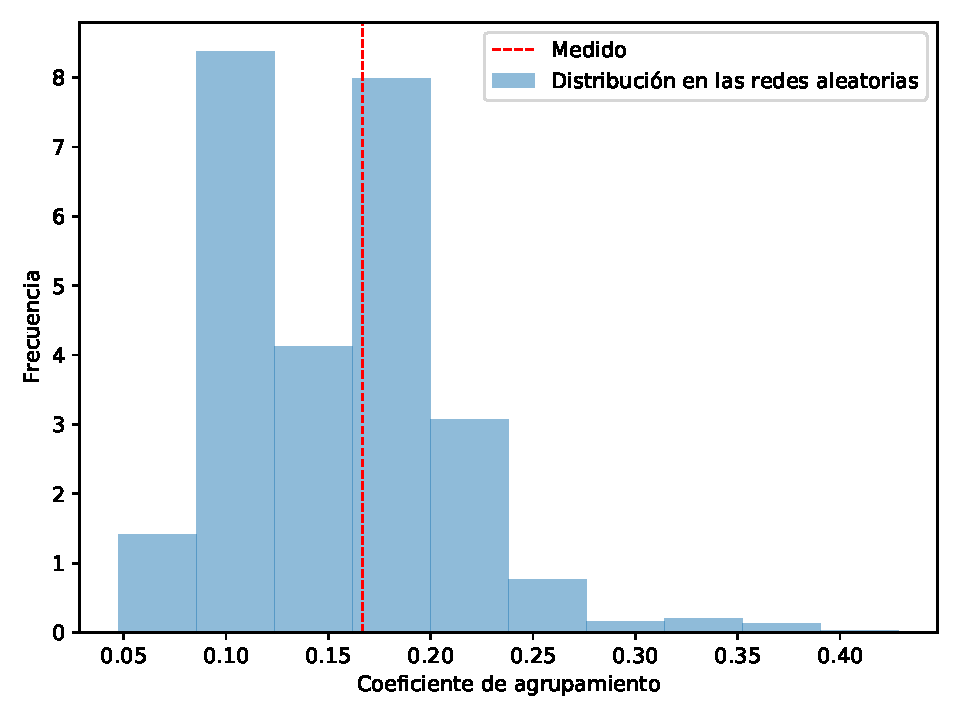
\includegraphics[width=\imsize]{Chap3/coef_clustering_distribucion.pdf}
        \caption[Distribución del coeficiente de agrupamiento en proyecciones de redes aleatorias.]{Distribución del coeficiente de agrupamiento calculado de las proyecciones en nodos tortugas de mil redes generadas aleatoriamente a partir de la red bipartita con datos de los tortugometros. En rojo está el valor medido del coeficiente de agrupamiento para la proyección en nodos tortugas (Fig. \ref{fig:proyeccion_red_campanas}).}
        \label{fig:distribucion_coef_agrupa}
       
        \end{center}
\end{figure}
 
\section{Proyecciones de redes bipartitas en nodos refugios}
Se realizaron las proyecciones de las redes bipartitas de refugios (Figs. \ref{fig:red_bipartita_refus_campanas} y \ref{fig:red_bipartita_refus_igotu}) en nodos refugios, Figs. \ref{fig:proyeccion_red_campanas_refus} y \ref{fig:proyeccion_red_igotu_refus}.
 
 
\begin{figure}[ht]
    \begin{center}
        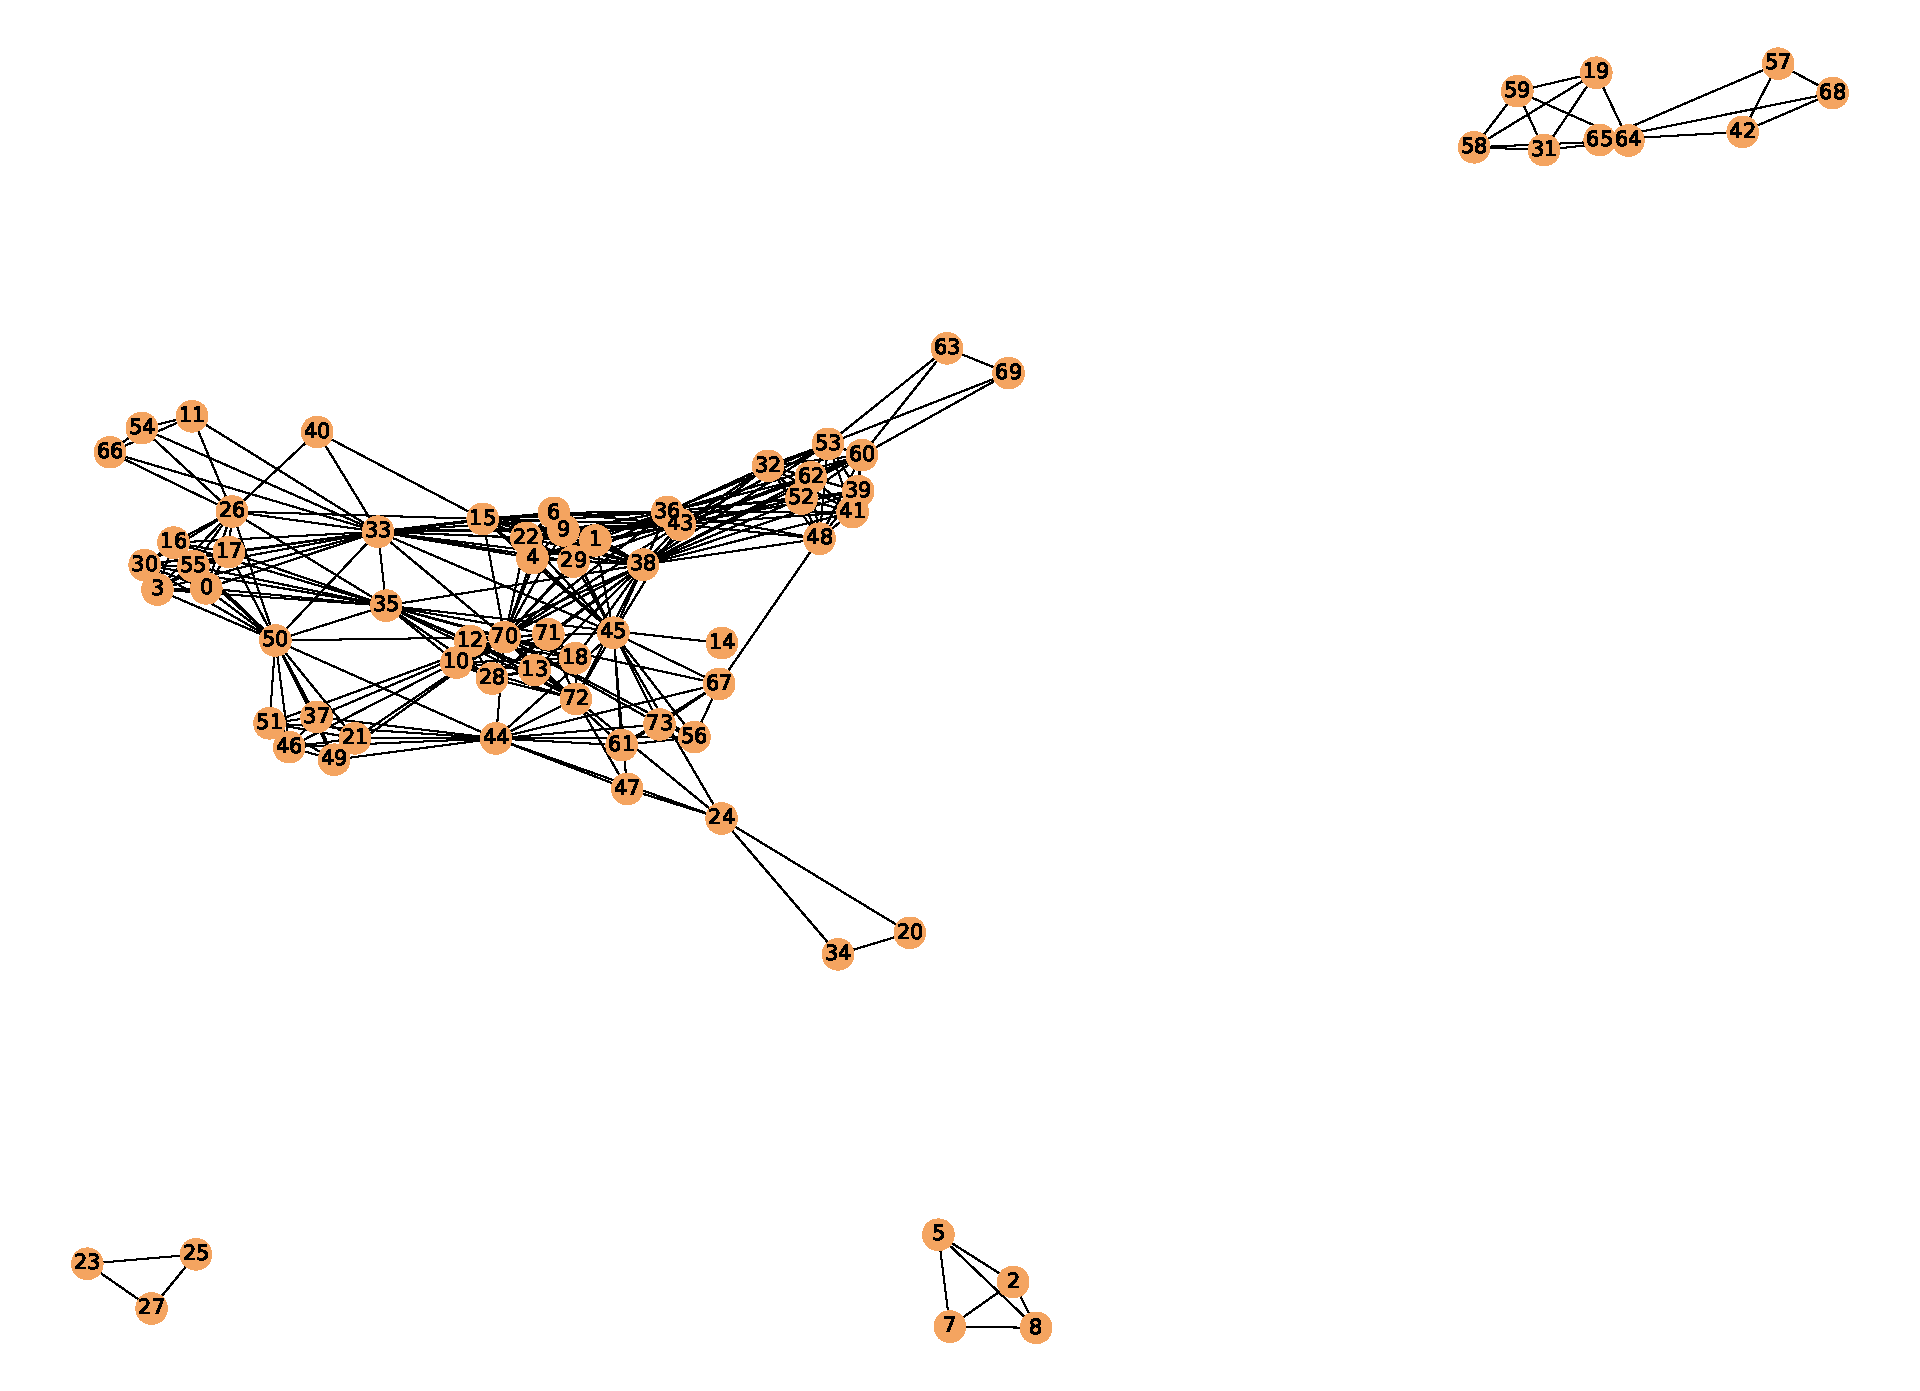
\includegraphics[width=\imsize]{Chap3/Proyecion_bipartita_ref_solo_ref.pdf}
        \caption[Proyección  de red bipartita de refugios para datos de los tortugometros en nodos refugios.]{Proyección  de red bipartita de refugios para datos de los tortugometros (Fig. \ref{fig:red_bipartita_refus_campanas}). Si hay una refugio compartido por un par de nodos tortugas, aparece una conexión entre este par de nodos en la proyección. }
        \label{fig:proyeccion_red_campanas_refus}
       
        \end{center}
\end{figure}
 
\begin{figure}[ht]
    \begin{center}
        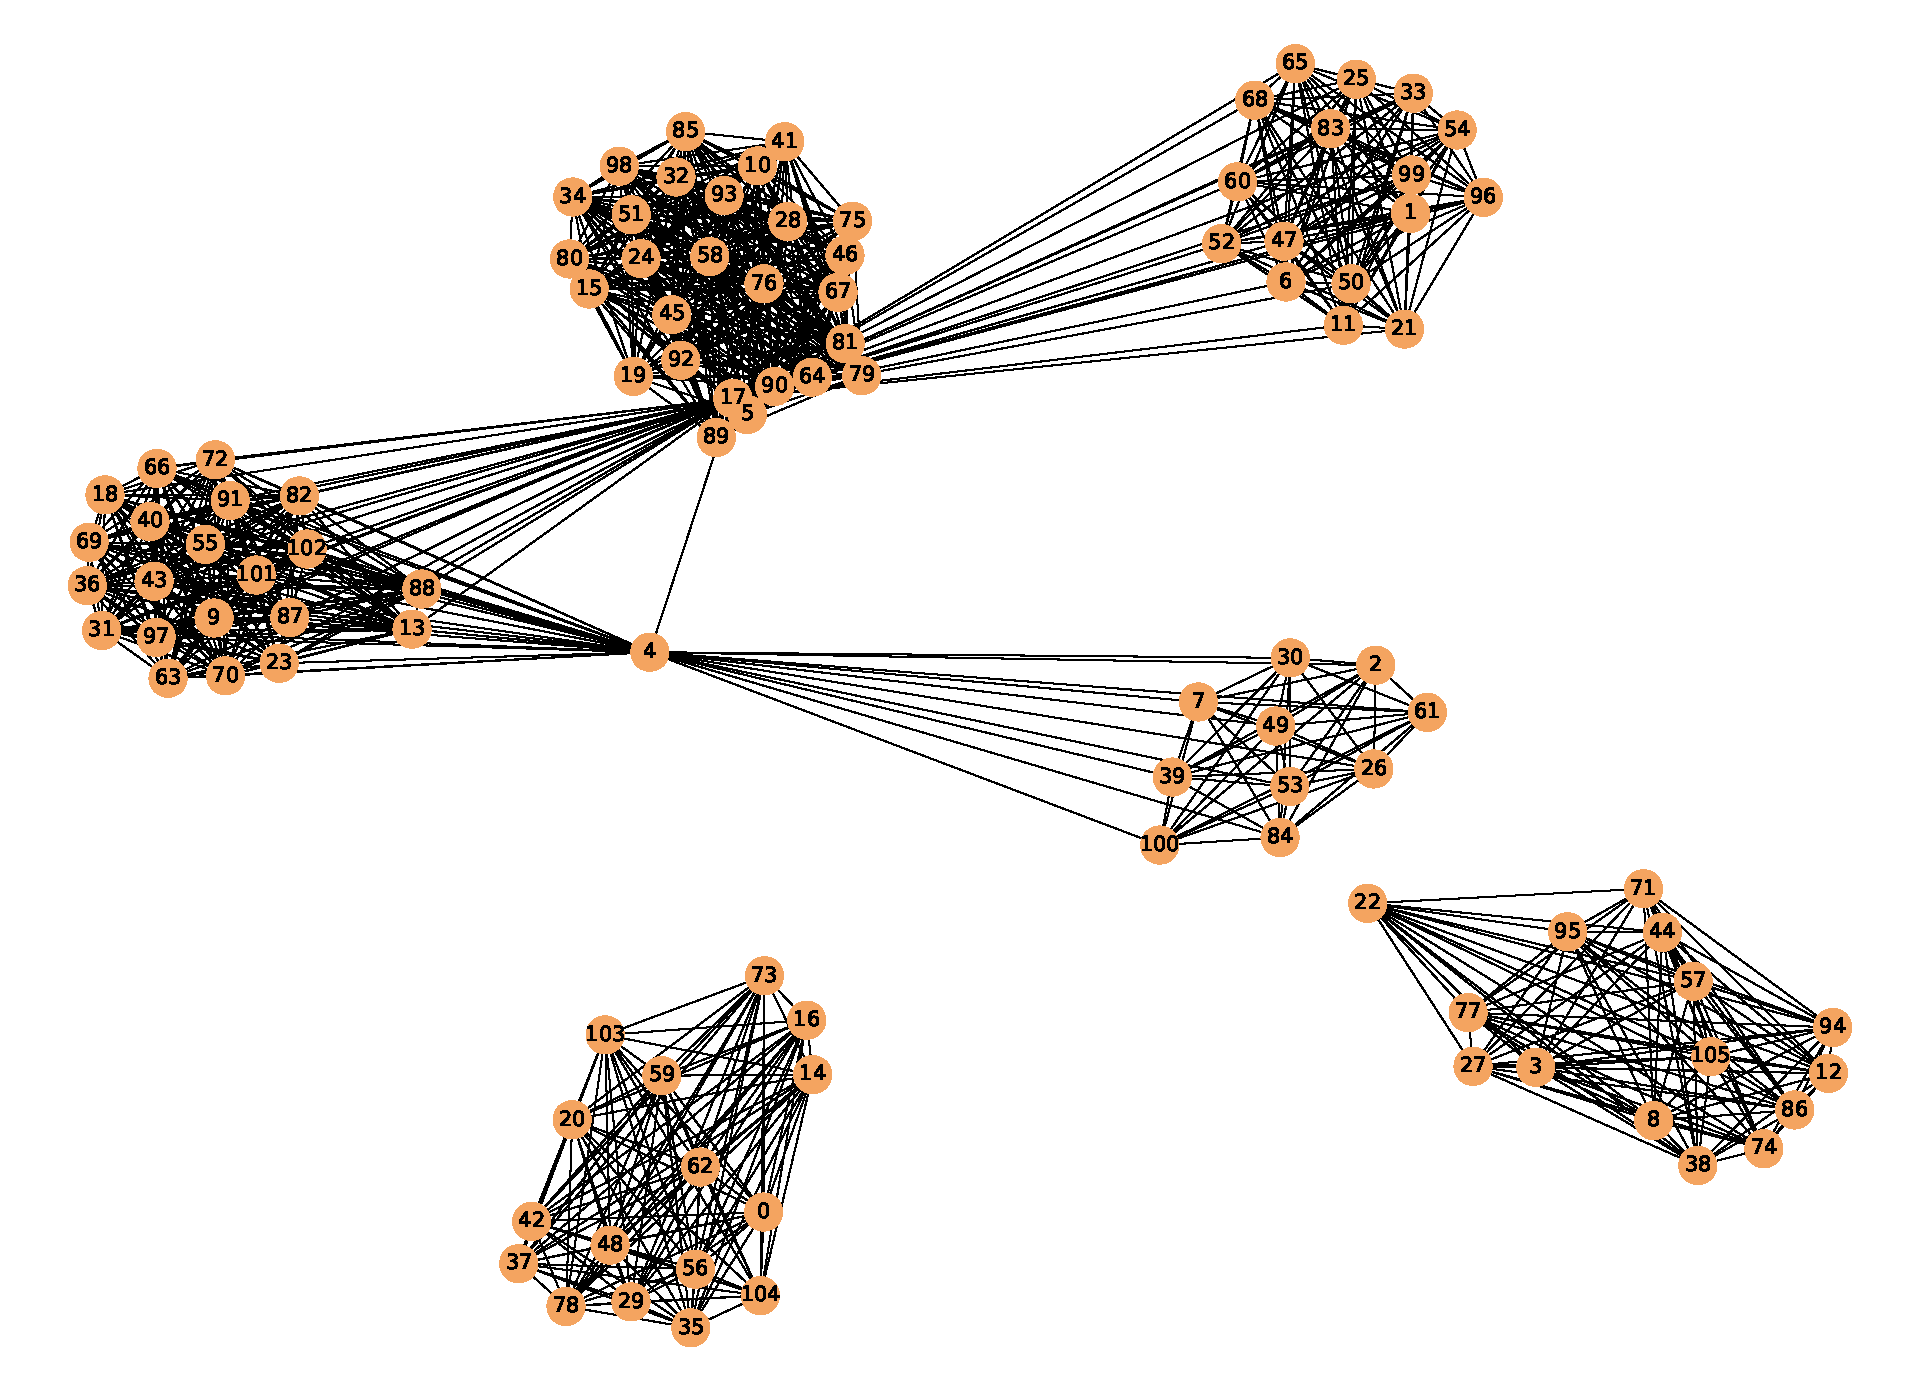
\includegraphics[width=\imsize]{Chap3/Proyecion_bipartita_ref_solo_ref_iGOTU.pdf}
        \caption[Proyección  de red bipartita de refugios para datos de los i-gotU en nodos refugios.]{Proyección  de red bipartita de refugios para datos de los i-gotU (Fig. \ref{fig:red_bipartita_refus_igotu}) sobre los nodos refugios. Si hay una refugio compartido por un par de nodos tortugas, aparece una conexión entre el refugio común con los respectivos refugios de ambas tortugas en la proyección. }
        \label{fig:proyeccion_red_igotu_refus}
       
        \end{center}
\end{figure}
Se observa en las Figs. \ref{fig:proyeccion_red_campanas_refus} y \ref{fig:proyeccion_red_igotu_refus}, pequeños clusters donde hay nodos completamente conectados (asociados a los refugios que visito una tortuga) con algunos nodos que conectan distintos clusters (asociados a algún refugio compartido). Ejemplo de este nodo conector es el refugio 4 (Fig. \ref{fig:proyeccion_red_igotu_refus}), que fue utilizado por la tortuga T30 y T6 en distintas noches (Fig. \ref{fig:red_bipartita_refus_igotu}).
 
Una pregunta subyacente de las proyecciones calculadas es si existe alguna relación entre los links formados y las distancias entre los nodos refugios. Para responder esta pregunta se graficaron los refugios en el mapa junto con las conexiones dadas por los links en las proyecciones. Un ejemplo de este mapa para los datos de los i-gotU se muestra en la Fig. \ref{fig:mapa_con_conexiones_igotu}. Se observa que parte de los links se encuentran entre refugios vecinos, pero también hay links entre refugios que se encuentran a distancias considerables respecto de refugios vecinos. A falta de una relación más rigurosa entre las distancias y los links, se realizó un \textit{mantel test} \cite{MantelTest} entre las matrices de adyacencia de las redes proyectadas en nodos refugios (Figs. \ref{fig:proyeccion_red_campanas_refus} y \ref{fig:proyeccion_red_igotu_refus}) con matrices de distancias entre refugios. En el lugar i,j de la matriz de distancias se encuentra la distancia entre el refugio  de la posición i y el refugio j (en metros) de la matriz de adyacencia.
 
El mantel test calcula el coeficiente de correlación de Pearson entre estas dos matrices, luego realiza permutaciones aleatorias de la matriz de distancias y vuelve a calcular el coeficiente de correlación de Pearson. El p-valor es la proporción de permutaciones que dan un coeficiente de correlación de Pearson mayor o igual al coeficiente de correlación de Pearson de la matriz de distancias original. Bajo la hipótesis de correlación nula en las dos matrices, las permutaciones aleatorias deberían ser igualmente probable de producir valores mayores o menores del coeficiente de correlación calculado.
 
 
Los mantel tests realizados con 10000 permutaciones aleatorias para los datos de los tortugometros y los i-gotU dan un p-valor de 0.0051 y 0.0001 respectivamente. Esto indica que existe una correlación significativa entre las distancias entre refugios y los enlaces en las redes proyectadas en nodos refugios (Figs. \ref{fig:proyeccion_red_campanas_refus} y \ref{fig:proyeccion_red_igotu_refus}). Es decir que la tortuga que visita un refugio, tiene una probabilidad mayor de visitar refugios cercanos a este, como se observa en la Fig. \ref{fig:mapa_con_conexiones_igotu}.
 
\begin{figure}[ht]
    \begin{center}
        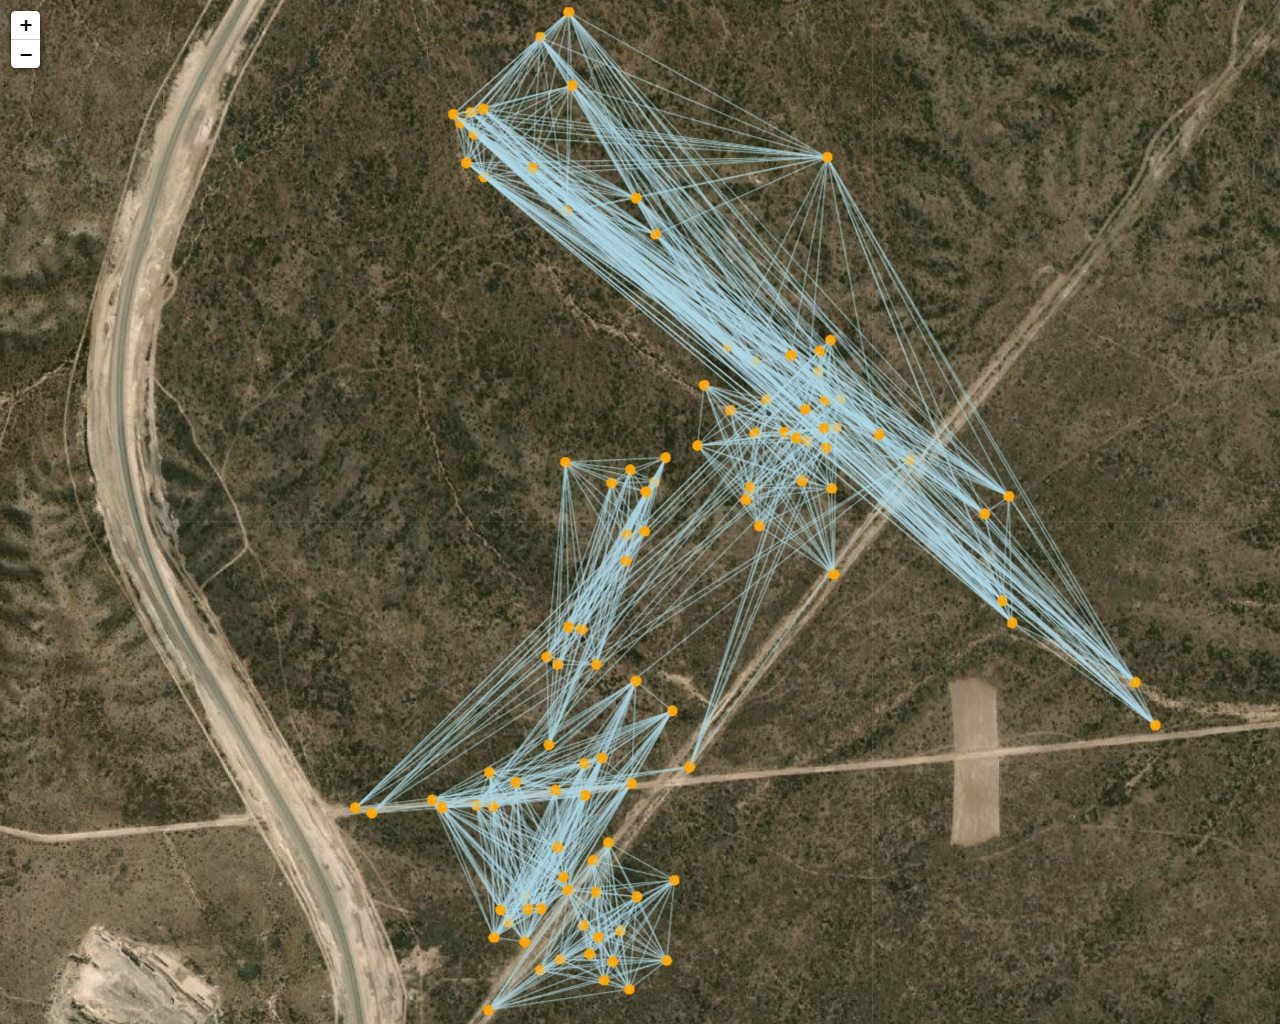
\includegraphics[width=\imsize]{Chap3/Mapa_refus_con_coneciones_igotu.jpg}
        \caption[Proyección en nodos refugios con conexiones en el mapa.]{Proyección de red bipartita (Fig. \ref{fig:proyeccion_red_igotu_refus}) en nodos refugios con conexiones en el mapa para los datos de i-gotU. }
        \label{fig:mapa_con_conexiones_igotu}
       
        \end{center}
\end{figure}
 
 
 
 
 
 


\chapter{Conclusiones y trabajo a futuro}
A partir de los resultados obtenidos en cada uno de los capítulos, 
se pueden enumerar las siguientes conclusiones:

\begin{itemize}

\item Se diseñó un algoritmo de reconstrucción de trayectorias, el mismo puede ser usado en cualquier especie indicando la velocidad máxima de la misma. Se encontró que la velocidad máxima de las tortugas es de 14 m/min. Fueron identificadas las zonas más visitadas por la población de tortugas estudiadas (Fig.~\ref{fig:grillaInt}), lo que podría ser útil para diseñar políticas de conservación. Los mapas de recurrencias podrán ser actualizados con nuevas mediciones y al devolver mapas en un formato html interactivo son de fácil uso para un trabajo interdisciplinario, en particular, durante las campañas.
 
\item Se obtuvieron redes  de interacción de individuos (Figs. \ref{fig:redInteraccion20mincampanas} y \ref{fig:redInteraccion20igotu}) y la cantidad de encuentros promedio para machos y hembras en los distintos meses de medición (Figs.~\ref{fig:encuentros_hora_medida_tortugometro} y \ref{fig:encuentros_hora_medida_igotu}). Se observa un pico para ambos sexos en noviembre-diciembre para los datos del tortugómetro, donde el 85\% de los encuentros registrados fueron hembra-macho, éste puede estar asociado a la búsqueda de pareja en la época de apareamiento. En el mes de enero las hembras presentan una mayor cantidad de encuentros promedio por hora medida que los machos (para datos de i-gotU y tortugometro), esta observación se estima que puede estar relacionada a la búsqueda de un lugar para sus huevos. De todas maneras, solo se contaron con 8 tortugómetros y 6 i-gotU  para cada día midiendo en simultáneo y es probable que parte de los encuentros no hayan sido registrados. En un futuro se analizará la red de interacciones aumentando el número de pares de individuos monitoreados.
 
 
\item Se definieron dos criterios para determinar el refugio donde pasó la noche la tortuga, uno para cada metodología de medición. Reconociendo las limitaciones de estos criterios, se decidió para las próximas campañas de medición aumentar las franja horaria de medición para los datos de i-gotU, de esta manera garantizar la ubicación de la tortuga en el refugio nocturno. Para el caso del tortugómetro se decidió añadir una etiqueta si la tortuga se encuentra en su refugio nocturno a la hora de recuperar el dispositivo en ese día de medición.
 
\item Con los refugios ya identificados, se definió una métrica para determinar la distribución espacial de los refugios en tortugas machos y hembras. Se observó que no presentan diferencias significativas entre machos y hembras, de todas maneras, el criterio utilizado para determinar un refugio para datos del tortugometro filtra muchos días de medición donde se le quitó el tortugómetro previo a las 20 horas. Por otro lado, los datos de i-gotU (donde tenemos una gran cantidad de refugios registrados) están tomados en los meses de enero-mayo, donde se espera una menor actividad de las tortugas machos (pasada época de apareamiento)\cite{Erika}.
 
\item Se identificaron en los refugios monitoreados por los i-gotU, donde tenemos días consecutivos de medición, la existencia de refugios preferidos (Fig. \ref{fig:refugios_preferidos}) donde la tortuga pasa la mayoría de las noches. En 4 de 6 tortugas monitoreados con metodología i-gotU, se encontró que realizan caminatas desde el refugio preferido hasta otro refugio nocturno y luego vuelven al refugio preferido. Un ejemplo de este último es la tortuga T54, en la red que manifiesta los caminos tomados (Fig. \ref{fig:ruta_refus_T54}), se observa que la tortuga  toma varias caminatas a otros refugios nocturnos y luego vuelve a alguno de sus dos refugios preferidos. Caracterizar estos refugios preferidos puede ser útil para diseñar políticas de conservación y puede además contribuir a la caracterización del movimiento, tanto para modelos matemáticos como simulaciones numéricas.
 
\item Partiendo de los refugios asociados a cada tortuga se armaron redes bipartitas de refugios y tortugas (Figs. \ref{fig:red_bipartita_refus_campanas} y \ref{fig:red_bipartita_refus_igotu}). Utilizando las proyecciones de los grafos bipartitos como predictor de enlaces en la red de encuentros, se encontró que para los datos de los tortugometros las métricas recall, precisión y accuracy no son mayores de lo esperado por uso de refugios aleatorio (tabla \ref{tab:metricas_comparacion_redes_aleatorias}). Para los datos de i-gotU, se observa que las métricas son mayores a las esperadas por uso de refugios aleatorios, pero se están monitoreando solo 6 tortugas y únicamente se encontraron 2 refugios compartidos entre las tortugas. Por poca cantidad de datos, no se puede aún afirmar si las proyecciones en la red bipartita nos dan una predicción de la red de encuentros.
 
\item Además, se compararon las topologías de las redes proyectadas en nodos tortugas con las redes de encuentros (tabla \ref{tab:metricas_topologia_redes}). Se observa que las redes bipartitas de refugios y tortugas tienen una topología similar a la red de encuentros, pero con una menor cantidad de enlaces y tampoco presentan diferencias significativas respecto el uso aleatorio de refugios.  En un futuro se analizará este razonamiento con una mayor cantidad de tortugas donde se disponga la misma cantidad de datos de refugios que de días de medición (condición que actualmente no se cumple para los datos del tortugometro).
 
\item Sobre las redes bipartitas de nodos tortugas y refugios, se realizaron proyecciones en nodos refugios (Figs. \ref{fig:red_bipartita_refus_campanas} y \ref{fig:red_bipartita_refus_igotu}) y se encontró que las matrices de adyacencia están fuertemente correlacionadas con la matrices de distancias. Se obtuvo un p-valor de 0.0051 y 0.0001, para los datos de los tortugometros y los i-gotU respectivamente, al realizar mantel tests con 10000 permutaciones aleatorias. Es decir que la tortuga que visita un refugio, tiene una probabilidad mayor de visitar refugios cercanos a este, como se observa en la Fig. \ref{fig:mapa_con_conexiones_igotu}.
 
\end{itemize}
 
 
 
 
 
 
 
 
%A partir de los resultados de este estudio, se decidió realizar en la próxima campaña un mayor esfuerzo de seguimiento de los individuos que participaron de los encuentros  detectados. De esta forma se busca entender si la no repetición de encuentros entre tortugas se debe a la poca cantidad de muestras o a una característica de la especie. Este resultado sería muy novedoso dado que está relacionado con la capacidad de memoria de las tortugas, un aspecto muy poco estudiado hasta el momento.
 
 
 
 



%\appendix
%\chapter{Ejemplo de ap\'{e}ndice: El problema de la medida \LGM{sacar/modificar}}\label{C:ap1}
\chapterquote{Negociemos Don Inodoro}{Fernando de la R\'{u}a, 2001}
\chapterquote{Smartness runs in my family.  When I went to school I was so smart my
teacher was in my class for five years}{George Burns}
\graphicspath{{figs/}}
%%%%%%%%%%%%%%%%%%%%%%%%%%%%%%%%%%%%%%%%%%%%%%%%%%%%%%%%%%%%%%%%%%%%%%%%
El gran problema lo constituye el proceso de medici\'{o}n. En la f\'{\i}sica cl\'{a}sica, medir significa revelar o poner de manifiesto propiedades que estaban en el sistema desde antes de que midamos \cite{Philipp1982NCBSp75}.

En mec\'{a}nica cu\'{a}ntica el proceso de medici\'{o}n altera de forma incontrolada la evoluci\'{o}n del sistema. Constituye un error pensar dentro del marco de la f\'{\i}sica cu\'{a}ntica que medir es revelar propiedades que estaban en el sistema con anterioridad. La informaci\'{o}n que nos proporciona la funci\'{o}n de onda es la distribuci\'{o}n de probabilidades, con la cual se podr\'{a} medir tal valor de tal cantidad. Cuando medimos ponemos en marcha un proceso que es indeterminable a priori, lo que algunos denominan azar, ya que habr\'{a} distintas probabilidades de medir distintos resultados. Esta idea fue y es a\'{u}n objeto de controversias y disputas entre los f\'{\i}sicos, fil\'{o}sofos y epistem\'{o}logos. Uno de los grandes objetores de esta interpretaci\'{o}n fue Albert Einstein, quien a prop\'{o}sito de esta idea dijo su famosa frase "Dios no juega a los dados".

Independientemente de los problemas de interpretaci\'{o}n, la mec\'{a}nica cu\'{a}ntica ha podido explicar esencialmente todo el mundo microsc\'{o}pico y ha hecho predicciones que han sido probadas experimentalmente de forma exitosa, por lo que es una teor\'{\i}a un\'{a}nimemente aceptada.

\begin{figure}[ht]
\centering{}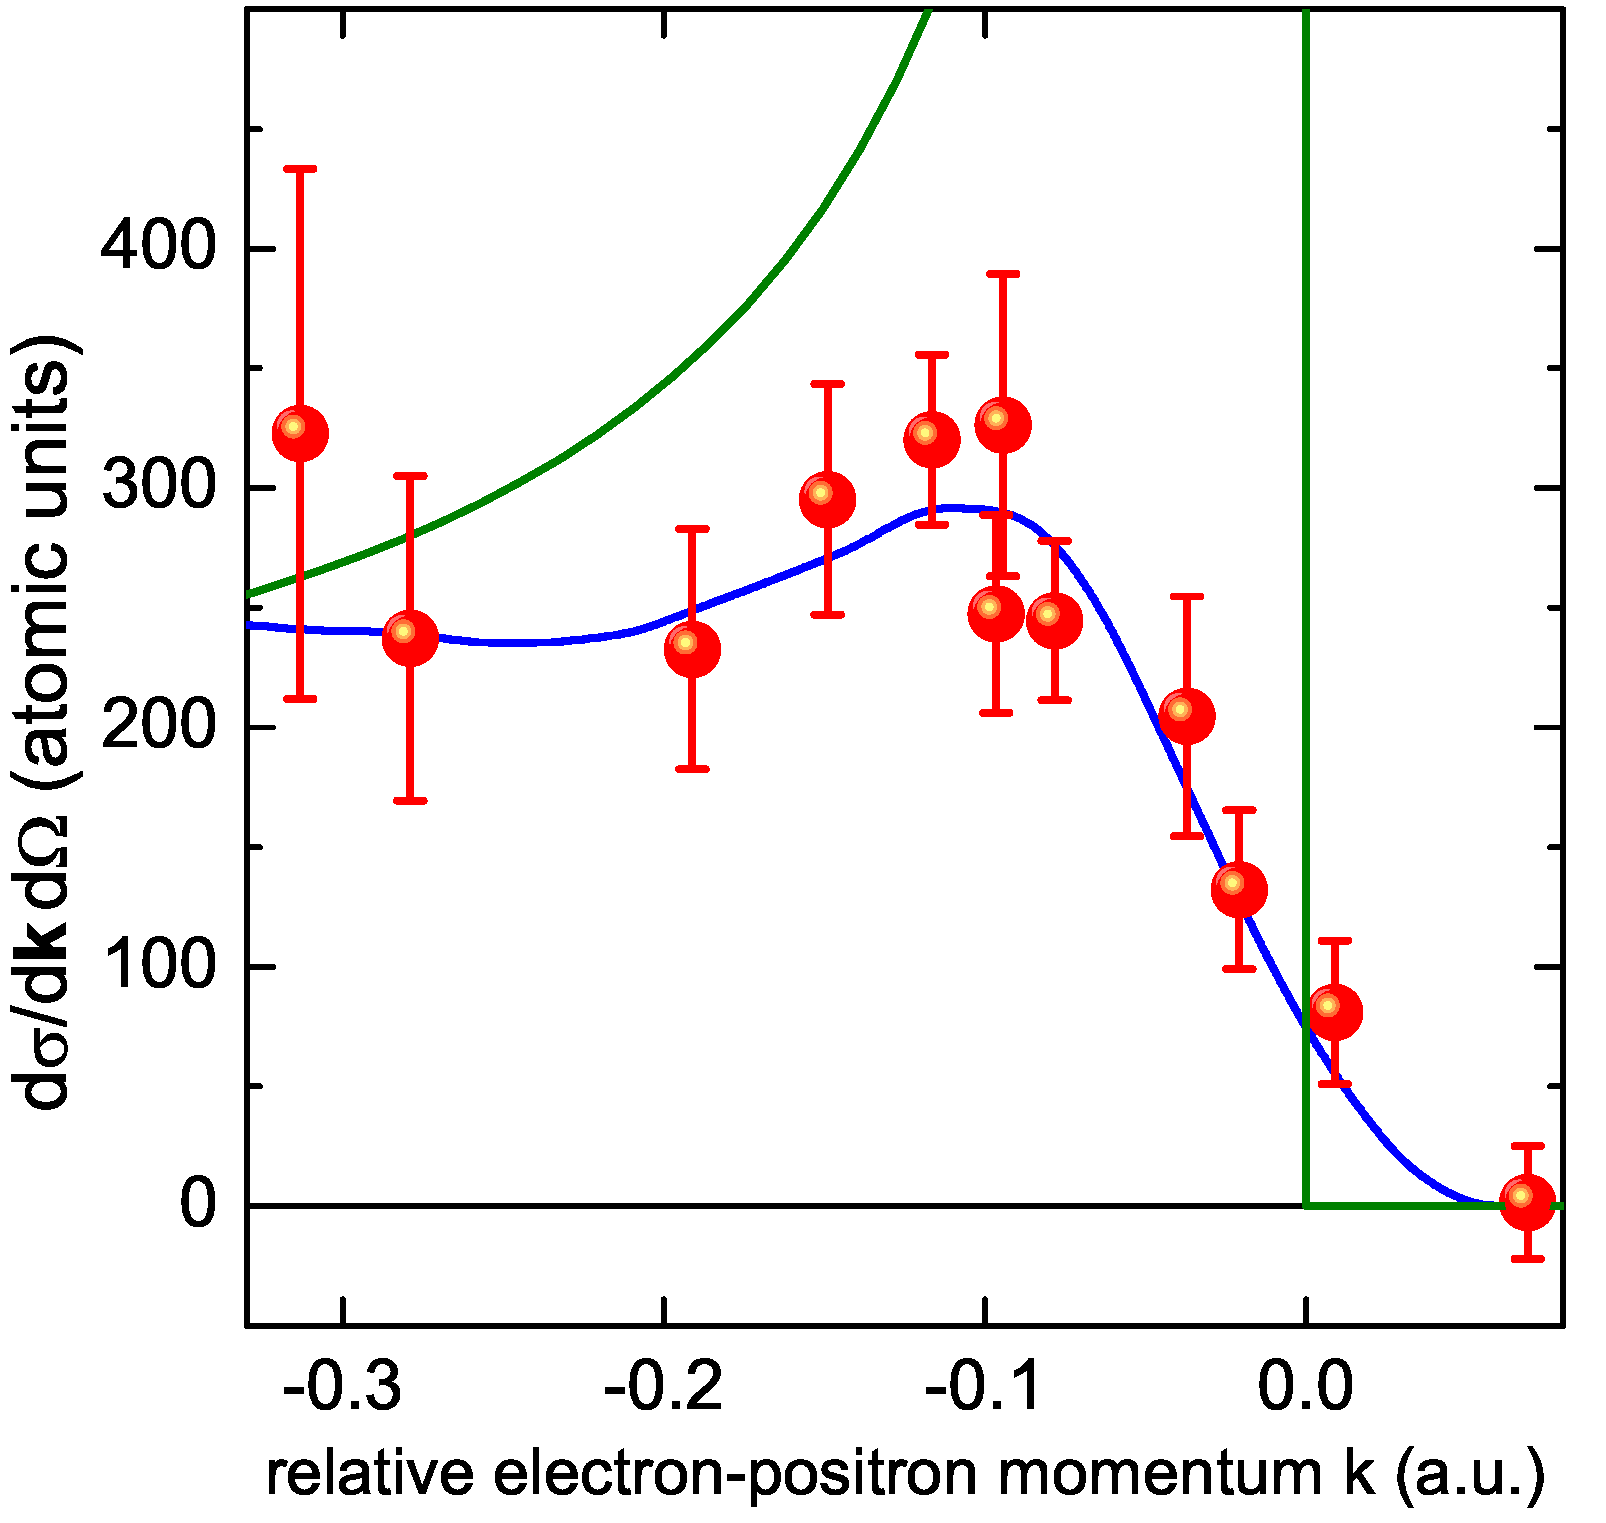
\includegraphics[width=\imsize]{ap1_f1}
\caption{Una figura con algunos puntos experimentales y curva de datos te\'{o}ricos\label{f:figura1}}  
\end{figure}



%%% Local Variables: 
%%% mode: latex
%%% TeX-master: "template"
%%% End: 


\begin{biblio}
\bibliography{mibib}
\end{biblio}


\begin{postliminary}

% \begin{seccion}{Publicaciones asociadas}
%   \begin{enumerate}
%   \item Mi primer aviso en la revista \textbf{ABC}, 1996
%   \item Mi segunda publicaci\'{o}n en la revista \textbf{ABC}, 1997
%   \end{enumerate}
% \end{seccion}

\begin{seccion}{Agradecimientos}
A Kari y Luis, por haber sido tan buenos directores y por haberme enseñado tanto. Ya sea en el aula (ML), en Git o en las numerosas reuniones que tuvimos durante el desarrollo de la tesis. La verdad la pasé muy bien tanto en la tesis como en laboratorio avanzado y eso tiene mucho mérito. También quería agradecer a todos las personas que participaron en las campañas de medición, haciendo mi tesis posible. \\

A mi mamá, por siempre estar para mí en todo momento, priorizando felicidad. En sus llamadas, dándome el apoyo emocional en caso de que sea necesario o simplemente mejorando mi día. No hubiera llegado a nada, en cada tropezón sé que la mejor idea es hablar con ustedes. \\

A mi papá, siempre apoyándome en mis decisiones y ayudándome a crecer como persona. Y por transmitirme su pasión por los animales y enseñándome a pensar como científico y hacerme tantas preguntas. No estaría acá si no fuera por esas tardes viendo como se incubaban los huevos de las gallinas araucanas y estoy más que agradecido por ello. \\

A mi abuela, por haberme abierto sus brazos en su casa los primeros años de carrera y todo su soporte para que hoy esté entregando esta tesis.\\

A Flor, por haberme bancado incondicionalmente, haberme regalado tantos momentos de calidad y por haberme acompañado en los últimos años. \\

A Tincho, Eze, Beani, Bata, Tebo, Fran, Ecu, Nico y Guate. Hicieron que mi vida universitaria fuera mucho más divertida, siempre una sonrisa en la cara. Me hicieron sentirme más que agradecido de haber entrado al Balseiro, son la familia que elegí. 
\end{seccion}

\end{postliminary}

\end{document}

